%\epigraphfontsize{\small\itshape}
%\setlength\epigraphwidth{8cm}
%\setlength\epigraphrule{0pt}
%\epigraphfontsize{\small\itshape}

%\epigraph{There are two possible outcomes: If the result confirms the hypothesis, then you've made a measurement. If the result is contrary to the hypothesis, then you've made a discovery.}{---\textup{ Enrico Fermi}}
%\epigraph{Everyone knows how useful it is to be useful. No one seems to know how useful it is to be useless.}{---\textup{  Chuang Tzu, The Useless Tree}}
\section{An Overview of the Reconstruction Algorithms in SNO+}
A particle interaction happens in the SNO+ detector can produce Cherenkov or scintillation photons. These photons propagate through the detector, and they can trigger PMTs when they reach the PSUP. As described in the last chapter, if there are enough PMTs triggered within a defined time window, an event is defined by the trigger system and for the event, the time and charge information measured by the hit PMTs are recorded.

By utilizing the recorded time and charge information, reconstruction algorithms attempt to calculate the physics quantities of an event, including its vertex (position and time), direction and energy. A few sets of reconstruction algorithms (called ``fitters'') have been implemented in the SNO+ RAT software or being developed. These fitters are based on different methods and they can be coordinated and optimized for the different detector situations or physics phases.

According to the physics quantities, the SNO+ fitters can be generally classified as:
\begin{itemize}
	\item Vertex fitter. A vertex fitter reconstructs the event position and time by utilizing the positions and timing information of the hit PMTs. Currently, vertex fitters have been used to process the data and simulations for the water and partial-fill phases. They are also ready for the scintillator and tellurium-loading phases.
	
    On the other hand, some particular events, such as radioactive background events emitting $\gamma$s, can create multiple vertices which are correlated. A multi-site or multi-vertex fitter will be useful for tagging and removing these events during the $0\nu\beta\beta$ search. This kind of fitter is being developed.

	\item Direction fitter. A direction fitter reconstructs the event direction by using the directional information from the Cherenkov photons, which cause ring-like patterns formed by the hit PMT positions. The direction fitter has been used in the water phase analysis. For the scintillator and tellurium-loading phases, since the Cherenkov patterns will be submerged in the scintillation photons, it requires the other efforts for the direction reconstruction, which is being developed currently. 
	
	\item Energy fitter. An energy fitter translates the number of photons created from an event to the kinetic energy. The optical response of each PMT, including the PMT detection efficiency, transmission probability, attenuation, and etc. Similar to the vertex fitters, the energy fitters currently have been used in the water and partial-fill phases, and they are ready for the scintillator and tellurium-loading phases.

	\item Muon track fitter. This fitter is used to reconstruct the tracks of cosmic muons. It treats a muon track as a straight line and by dividing the SNO+ detector into several XY-slices along z, it reconstructs the intersection points for each slice by utilizing the positions and timing information of the hit PMTs\cite{muonTrackRecon}. It is currently being developed for the scintillator and tellurium-loading phases. It will help to tag and reduce the cosmogenic backgrounds, especially the $^{11}$C backgrounds induced by the muon spallation on the liquid scintillators\cite{sorensen2016temperature}.
\end{itemize}

For a fitter, its performance is first tested on the Monte Carlo simulations of specific physics processes. Then it is tested on both the simulations and real data of the calibration runs. Once the algorithm gives proper results which are approved by the collaboration, it is implemented into the SNO+ RAT software to process the SNO+ simulations and data files.

For a specific SNO+ physics phase, the fitters for different physics quantities of an event are integrated together. Currently, there are three integrated fitters: the \texttt{Water Fitter} for the water phase, the \texttt{Partial Fitter} for the partial-fill phase and the \texttt{Scint Fitter} for the scintillator phase and the tellurium loading phase. The fitter parameters, such as the input optical parameters, fitter iterations, are coordinated and optimized based on simulations and calibration data from that specific physics phase. 

PMT selectors and classifiers are also wrapped into the integrated fitters. The PMT selectors are used to remove the outliers of the hit PMTs for a specific fitter, such as the hit PMT probably triggered by the noises. These selectors can help to make the fitter more accurate or to boost up the algorithm speed of the fitter. The classifiers mainly use the reconstructed results to calculate some specific quantities which describe the probability of an event being a specific signal or background.

In this chapter, a Multi-path (MP) reconstruction framework is discussed. It was developed by the University of Alberta group as an additional fitter to provide event vertex and direction reconstructions. In this framework, the fitters are able to be adapted for all the SNO+ physics phases by switching light path calculations as well as the input optical parameters, that is the reason why it is called "multiple paths". It was applied in the water phase to provide alternative information of the event position and direction; it also works as the vertex reconstruction algorithm for the \texttt{Partial Fitter}. After re-coordination to the scintillator phase and tellurium loading phase, I also show the potentials of the vertex fitter being applied in these two future phases.

Besides, potentials of extracting the directional information from the scintillator phase is discussed.
\section{Multi-path Reconstruction Algorithm for SNO+}\label{sect:mpw}

In the SNO+ water phase, the cavity and the AV are both filled with ultra-pure water. This is a relatively simple geometry since everything inside the PSUP can be simplified as water. Therefore, I will start with the MP water fitter (the MPW fitter) to explain the reconstruction concepts.

The MPW fitter fits for position, time and direction of a triggered event in SNO+ water phase. First, the fitter throws a random position built up by random variables which are uniformly distributed inside a sphere with a radius of $10~meters$ (larger than the actual PSUP radius $r_{PSUP}=8.39~m$). Meanwhile, a random event time is also generated, following a uniform distribution in a range of $100$ to $300~ns$. The Class Library for High Energy Physics (\texttt{CLHEP}) is used for creating pseudo-random numbers (see the Appendix A.1 for details). The random position and the random time are combined to form a random event vertex, which is set as the trial event vertex.

For a triggered event, photons are created around the event position and propagate to the PMTs.
In a simplified situation neglecting reflection and refraction, these photons propagate along straight line. Connecting the trial event vertex to the hit PMTs, the fitter evaluates a timing parameter, called the time residual ($t_{res}$), which is defined as:
\begin{equation}
\label{tres_define}
t_{res}=t_{PMT} - t_{transit} - t_{event},
\end{equation}

where $t_{PMT}$ is the PMT trigger time recorded by the detector, $t_{event}$ is the time when an event occurs (event time), and $t_{transit}$ is the total transit time (or time of flight, $TOF$) taken by a photon traveling from the event position ($\vec{x}_{event}$) to the hit PMT ($\vec{x}_{PMT}$) and crossing different materials in the detector.

To calculate the $t_{transit}$, the fitter uses photons from prompt time window (prompt light) and assumes that photons propagate in straight lines (straight light paths). The simple straight light path calculation gives $t_{transit}=|\vec{x}_{event}-\vec{x}_{PMT}|/v_{water}$. Detailed calculations, such as refraction and reflection when the lights cross different detector materials, absorption and scattering from the materials, as well as the lensing effects caused by the spherical structure of the acrylic vessel, are neglected. It was found that without these details, the fitter can still produce decent results that are consistent with the ones using detailed calculations. 

For a trial vertex $(\vec{x}_0,t_0)$, the fitter calculates a set of $t_{res}$ values with respect to all the hit PMTs. These values are fed into a likelihood function: 
\begin{equation}
\ln\mathcal{L}(\vec{x}_0,t_0)=\sum_{i=1}^{{\mathrm{Nhits}}}\ln P(t^i_{res}),
\end{equation}
where $t^i_{res}$ is the time residual calculated from the $i^{th}$ hit PMT and $\mathrm{Nhits}$ here stands for the number of total hit PMTs by an event.

A pre-set 1-dimensional (1D) probability density function is used for fitting the model. The $pdf$ was taken from the bench-top timing profile measurement as well as the measured detector response.

$P(t^i_{res})$ is the probability returned from the $pdf$ for the $i^{th}$ hit PMT and a trial event vertex.

The Levenberg-Marquardt method, which is commonly used for fitting the nonlinear model for multiple parameters, is used as an optimizer to find the best fit event parameters (position, time and direction). Appendix A.2 describes this method; A.3 describes the implementation of the method to the MultiPath fitter framework. Also see \cite{gregory2005bayesian, press2007numerical}.

As will be shown in the following sections, one of the main tasks for the fitter is to calculate the $t_{transit}$ by evaluating light paths. In the water phase, photons created in an event were considered as traveling along straight line paths and these paths are always in the water, i.e., the paths inside the AV or other detector components were not taken into account. In the other situations, for example, when the acrylic vessel is filled with the wavelength shifter or scintillator, the light path calculations will be modified.   

Fig.~\ref{mpwdiagram} shows the reconstruction concepts for position and direction.
\begin{figure}[htbp]
	\centering
	\begin{minipage}[t]{0.45\textwidth}
		\centering
		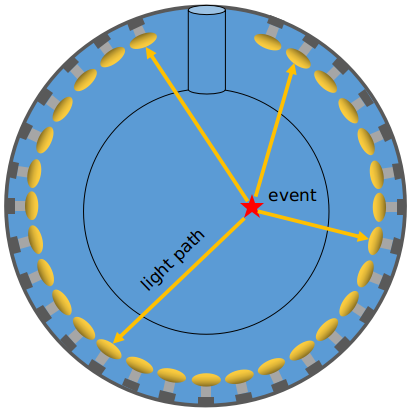
\includegraphics[width=5cm]{mpwDiagram.png}
	\end{minipage}
	\begin{minipage}[t]{0.4\textwidth}
		\centering
		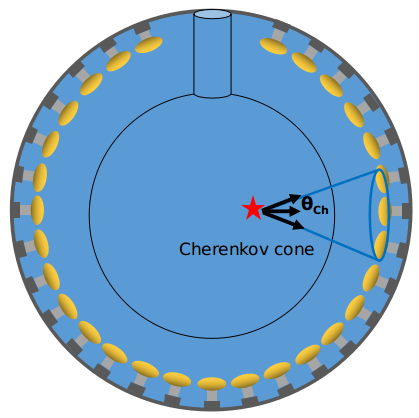
\includegraphics[width=5cm]{mpwDiagram2.png}
	\end{minipage}
	\caption{Diagrams of position (left) and direction (right) reconstruction in SNO+ water phase.}
	\label{mpwdiagram}
\end{figure}
	
\section{Multi-path Position and Direction Reconstructions for the Water Phase}

\subsection{Vertex Reconstruction}
For the position reconstruction of the MPW fitter, the likelihood function simply calculates the likelihood assuming straight line paths of prompt light from a position vertex $\vec{X_0}$ ($\mathrm{fVertex}$) and a starting time offset $t_0$ to each of the hit PMTs. 

The position difference is defined as $\vec{X}_{{\mathrm{diffCh}}} = \vec{X_0}-\vec{X}_{\mathrm{pmt}}$. Then the time of flight for prompt light is $t_{\mathrm{Ch}}=|\vec{X}_{{\mathrm{diffCh}}}|/v_g$ and $L_{\mathrm{Ch}}=L(t_{\mathrm{Ch}})$.

The derivatives of the likelihood function can be calculated from explicit mathematical forms as:
\[
\frac{\partial L}{\partial t_0}=\frac{dL_{\mathrm{Ch}}}{dt_{\mathrm{Ch}}},
\]

\[
\frac{\partial L}{\partial x}=\frac{\partial L_{\mathrm{Ch}}}{\partial t_{\mathrm{Ch}}}\frac{dt_{\mathrm{Ch}}}{\partial x}=-\frac{dL_{\mathrm{Ch}}}{dt_{\mathrm{Ch}}}\frac{X_{{\mathrm{diffCh}}}}{|\vec{X}_{{\mathrm{diffCh}}}|\cdot v_g},
\]

\[
\frac{\partial L}{\partial y}=-\frac{dL_{\mathrm{Ch}}}{dt_{\mathrm{Ch}}}\frac{Y_{{\mathrm{diffCh}}}}{|\vec{X}_{{\mathrm{diffCh}}}|\cdot v_g},
\]

\[
\frac{\partial L}{\partial z}=-\frac{dL_{\mathrm{Ch}}}{dt_{\mathrm{Ch}}}\frac{Z_{{\mathrm{diffCh}}}}{|\vec{X}_{{\mathrm{diffCh}}}|\cdot v_g},
\]

where $\frac{dL_{\mathrm{Ch}}}{dt_{\mathrm{Ch}}}$ can be calculated numerically from the timing $pdf$. 

In the WaterPosition class, it starts with a random ($\vec{x}_0,t_0$) as seed and calculates the likelihoods and their derivatives for various paths. These values are sent to the Multi-path Fitter, which is fitting 4 parameters: $x,y,z,t$ and to maximize the likelihood function through the MRQ method and to find the best-fit positions.


\begin{figure}[!htb]
	\centering
	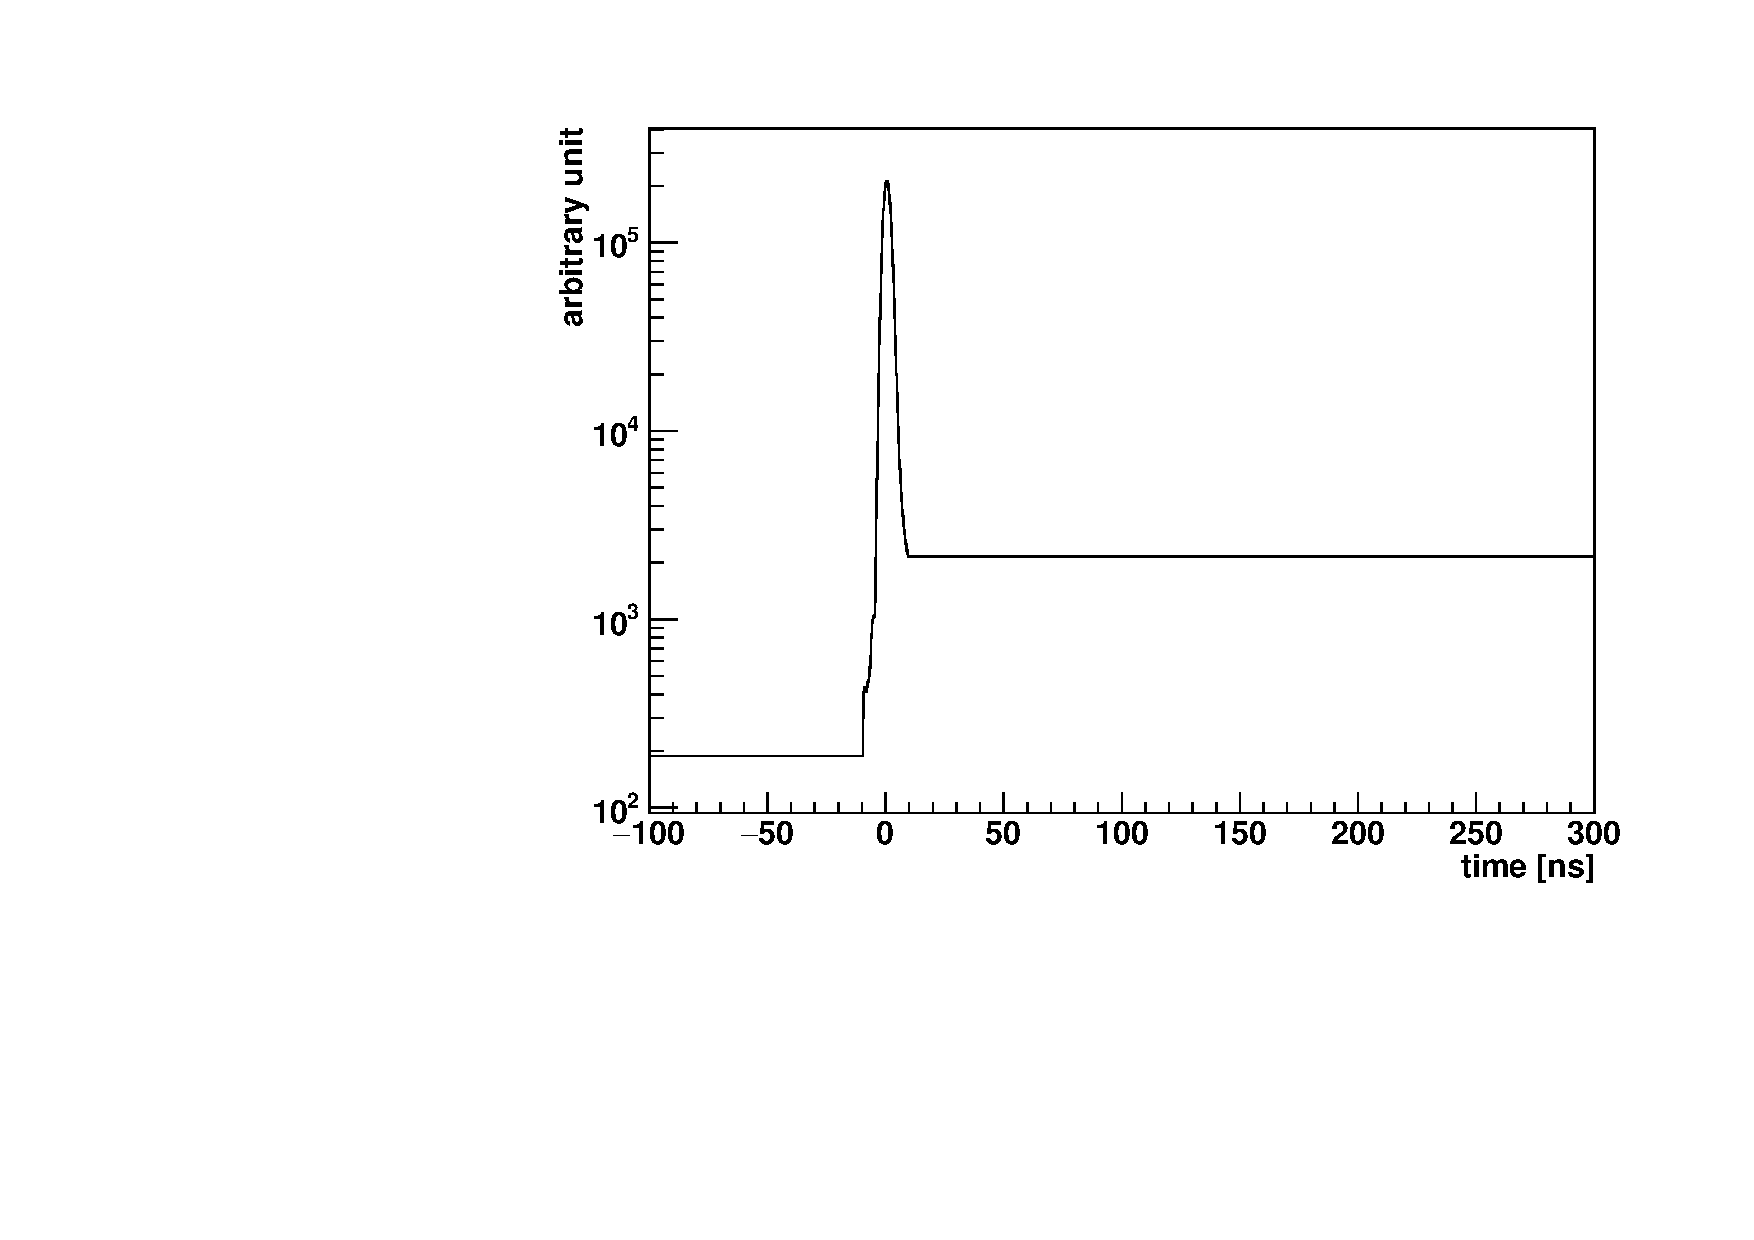
\includegraphics[width=10cm]{MPW_timingPDF.pdf}
	\caption{PMT response time as the timing $pdf$ for vertex reconstruction.}
	\label{MPW_timingPDF}
\end{figure}



\begin{figure}[!htb]
	\centering
	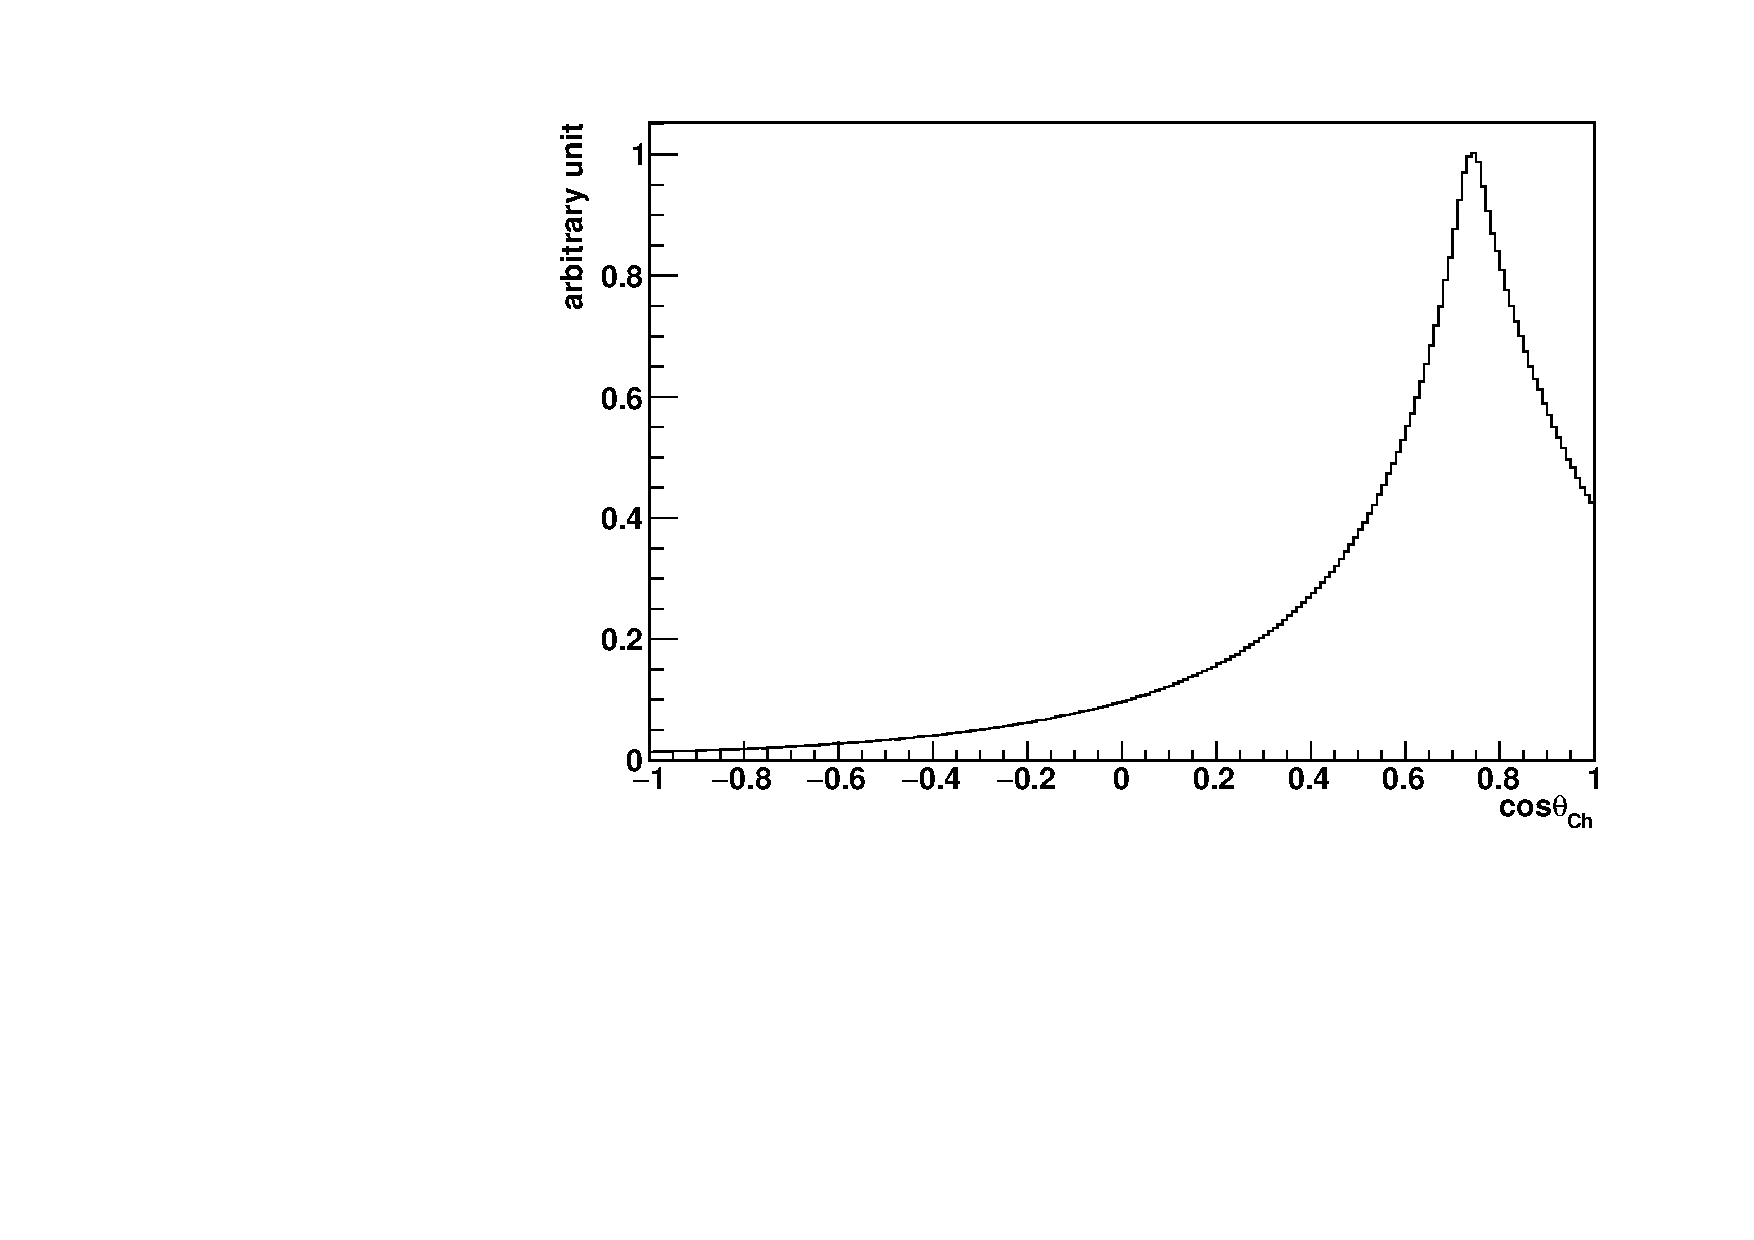
\includegraphics[width=10cm]{MPW_angularPDF.pdf}
	\caption{PMT angular distribution as the angular response $pdf$ for direction reconstruction.}
	\label{MPW_angularPDF}
\end{figure}

\subsection{Direction Reconstruction}
 $\vec{u}_{0}=(\cos\phi\sin\theta,\sin\phi\sin\theta,\cos\theta)$ ($\mathrm{fDirection}$), where the $\theta$ is zenith angle and $\phi$ the azimuth. $\cos\theta_{\mathrm{Ch}}$ is the angle between $\vec{u}_{0}$ and $\vec{X}_{{\mathrm{diffCh}}}$, which is taken as the fitting parameter of the likelihood function for the direction reconstruction. For the i-th hit PMT, $\cos\theta^i_{\mathrm{Ch}}=\vec{u}_0\cdot\frac{\vec{X}^i_{{\mathrm{diffCh}}}}{|\vec{X}^i_{{\mathrm{diffCh}}}|}$, then the likelihood function is:
\[
L(\vec{u}_0)=\sum_{i=1}^{{\mathrm{Nhits}}}L_i(\cos\theta_{\mathrm{Ch}}^i),
\]

The derivatives have explicit mathematical forms:
\[
\frac{\partial L}{\partial\theta}=\frac{dL_{\mathrm{Ch}}}{d\cos\theta_{\mathrm{Ch}}}\frac{d\cos\theta_{\mathrm{Ch}}}{\partial\theta}
=\frac{dL_{\mathrm{Ch}}}{d\cos\theta_{\mathrm{Ch}}}\frac{d\vec{u}_0}{d\theta}\cdot\frac{\vec{X}_{{\mathrm{diffCh}}}}{|\vec{X}_{{\mathrm{diffCh}}}|},
\]
where $d\vec{u}_0/d\theta=(\cos\phi\cos\theta, \sin\phi\cos\theta, -\sin\theta)$ and 
\[
\frac{\partial L}{\partial\phi}=\frac{dL_{\mathrm{Ch}}}{d\cos\theta_{\mathrm{Ch}}}\frac{d\cos\theta_{\mathrm{Ch}}}{d\phi}
=\frac{dL_{\mathrm{Ch}}}{d\cos\theta_{\mathrm{Ch}}}\frac{d\vec{u}_0}{d\phi}\cdot\frac{\vec{X}_{{\mathrm{diffCh}}}}{|\vec{X}_{{\mathrm{diffCh}}}|},
\] where $d\vec{u}_0/d\phi=(-\sin\phi\sin\theta, \cos\phi\sin\theta, 0)$. $\frac{dL_{\mathrm{Ch}}}{d\cos\theta_{\mathrm{Ch}}}$ can be calculated numerically from the PMT angular response pdf.

In the FitterWaterDirection class, it starts with a random ($\theta_0,\phi_0$) as seed and calculates the likelihoods and their derivatives for various paths. These values are sent to the Multi-path Fitter, which is now fitting 2 parameters: ($\theta,\phi$) and to maximize the likelihood function through the MRQ method and to find the best-fit directions.

\subsection{Effective Group Velocity}\label{tuneGroupVelocity}
When photons travel through the detector, their group velocities change with different refractive indices of different detector materials. The group velocities also depend on the wavelengths of the photons as $v_g=c/n(\lambda)$. Fig~.\ref{nVsWavelength} shows the measured refractive indices as a function of wavelength, obtained from the measurements of laserball scans in the SNO+ water phase\cite{laserball_groupVelocity}. Furthermore, the group velocities can change when these photons are scattered, absorbed, refracted and reflected. To simplify these complicated situations for the reconstruction, an averaged value of the group velocity is used in the straight line light path calculation. This fixed group velocity is considered as an effective value.

\begin{figure}[!htb]
	\centering
	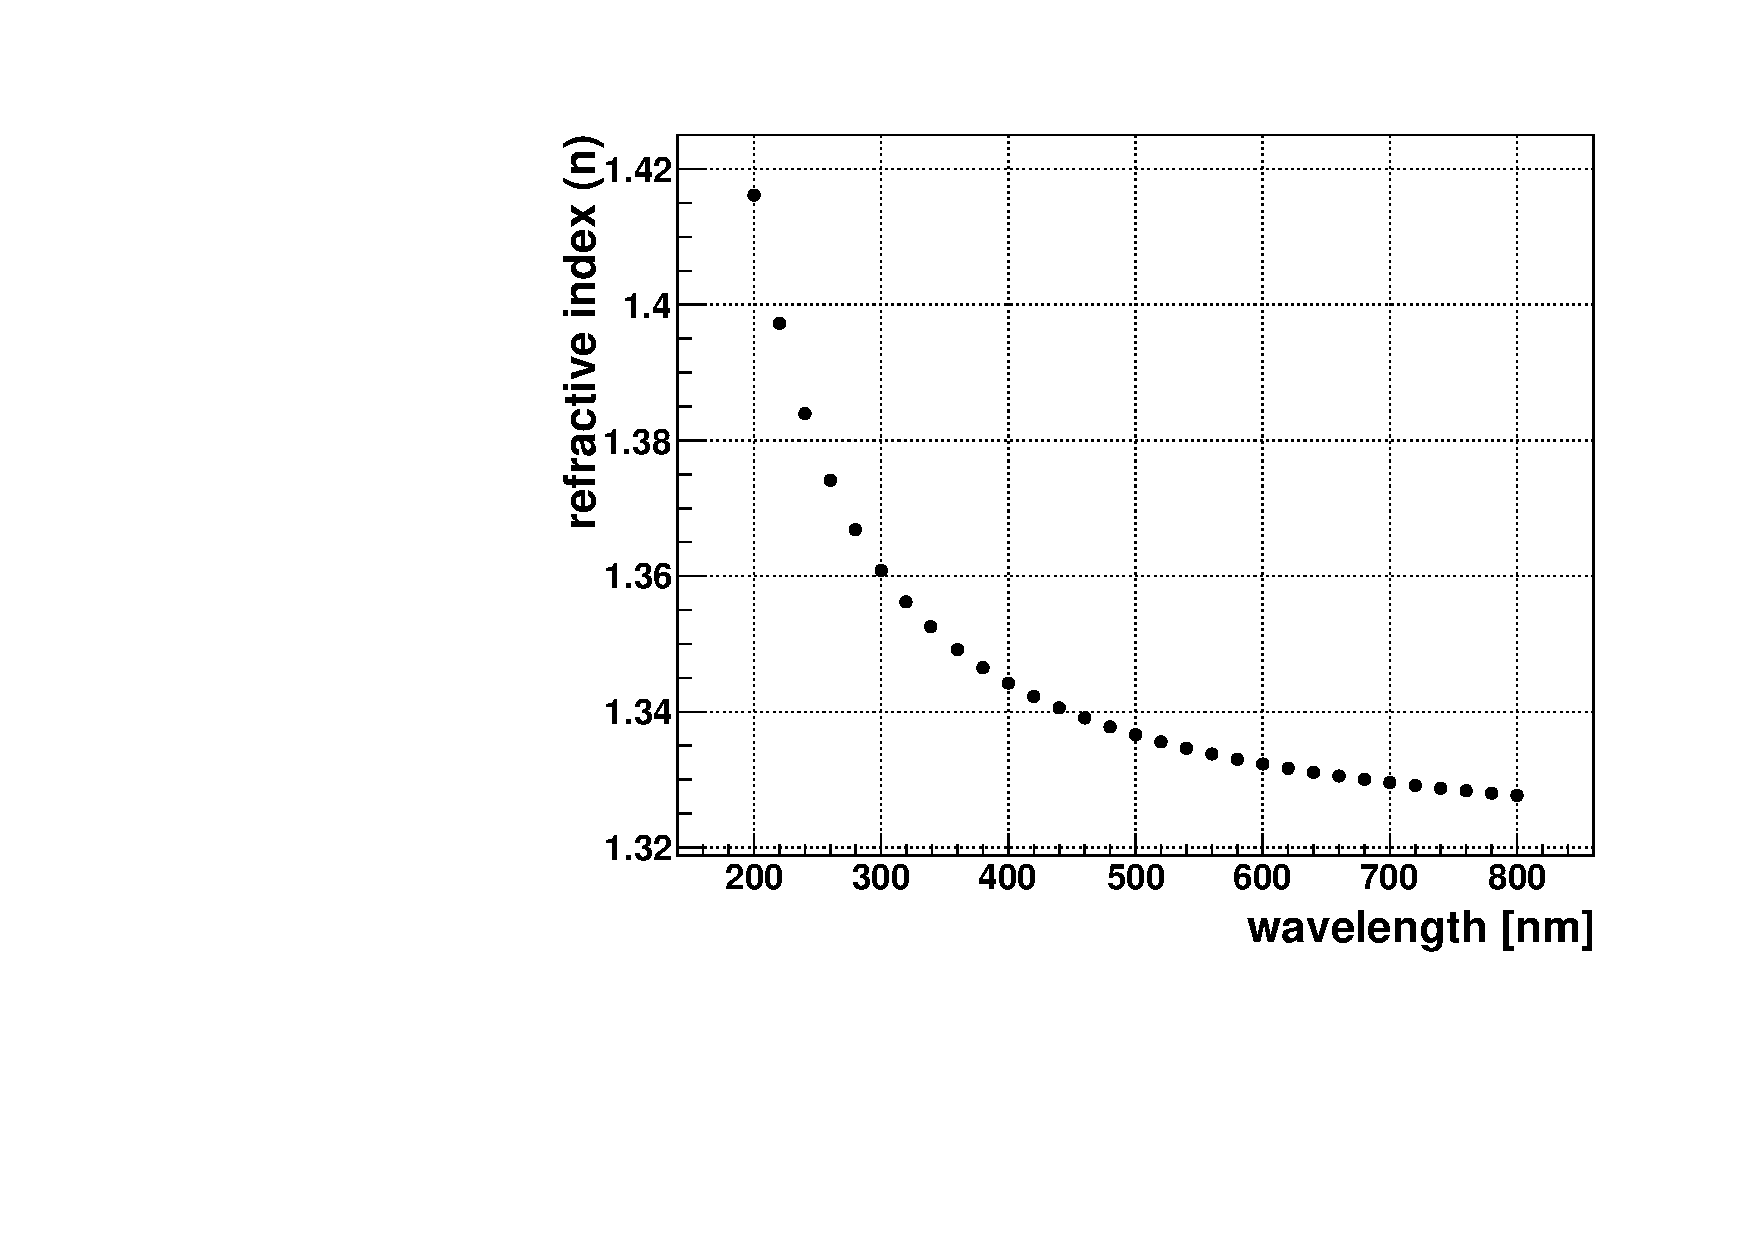
\includegraphics[width=6cm]{refractiveIndexVsWavelength.pdf}
	\caption{Refractive index vs wavelength. These values are based on the measurements from laserball calibration scans in the SNO+ water phase\cite{laserball_groupVelocity}.}
	\label{nVsWavelength}
\end{figure}

A reasonable selection of this value is required, since the value can introduce biases in the fitted position. This kind of bias is mainly due to a ``complementary'' effect of the fitter. As mentioned in section \ref{sect:mpw}, the water vertex fitter calculates the $t_{transit}$ by evaluating the distances from the trial vertex to the hit PMTs: $t_{transit}=|\vec{x}_{event}-\vec{x}_{PMT}|/v_{water}$. If the value of the group velocity $v_{water}$ is set large (or fast speed), the value of $t_{transit}$ will decrease, and the corresponding value of $t_{res}$ will increase according to the definition of $t_{res}$(\ref{tres_define}). These calculated $t_{res}$ value is compared to the time pdf for the fitting. If $t_{res}$ is larger than the expected value, the fitter will place the trial vertex away from the 
hit PMTs to increase the $t_{transit}$ and then decrease the $t_{res}$, as illustrated in Fig.~\ref{effectiveVg}. On the other hand, if $v_{water}$ is set small (or slow speed), $t_{transit}$ increases and $t_{res}$ decreases, and the fitter will place the trial vertex closer towards the hit PMTs.
Therefore, an overestimated group velocity (too fast) brings a positive radial bias to the true event position while an underestimated one (too slow) brings a negative radial bias.
\begin{figure}[!htb]
	\centering
	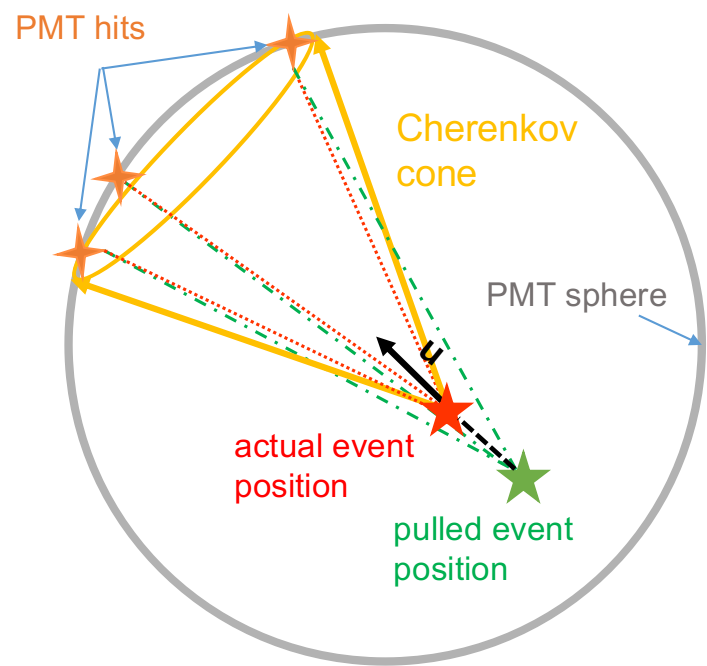
\includegraphics[width=6cm]{effectOfGroupVelocity.png}
	\caption{A cartoon shows effects of tuning the effective group velocity. In this case, the effective group velocity is faster than expected, the fitted position is dragged back along the direction to increase the time of flight.}
	\label{effectiveVg}
\end{figure}

In practice, the effective group velocity is tuned by an effective refractive index $n_{eff}$ (or called $RI$ value): $v_{water}=c/n_{eff}$. To select a reasonable effective group velocity for the water-phase vertex fitter, my first approach is to test on all the values of the refractive index provided by the SNO+ laserball measurements. The values are listed in Fig.~\ref{nVsWavelength}. 


I choose the one which gives the smallest radial bias based on MC simulations. 
For typical 5 MeV $e^-$ events simulated uniformly inside the AV and isotropic momentum,  

As shown in Fig.~\ref{plotGroupV}, $n_{eff}=1.40$ gives the smallest radial bias and is adopt for the MC case.

%\begin{figure}[!htb]
%	\centering
%	\includegraphics[width=6cm]{}
%	\caption{Biases .}
%	\label{plotGroupV}
%\end{figure}

Later I turned to a more data-driven approach rather than just tuning from the simulations. This approach is to extract an average group velocity by analyzing the $^{16}$N calibration source data.

as shown in Fig.~\ref{n16_groupVeloctiy}.

\begin{figure}[!htb]
	\centering
	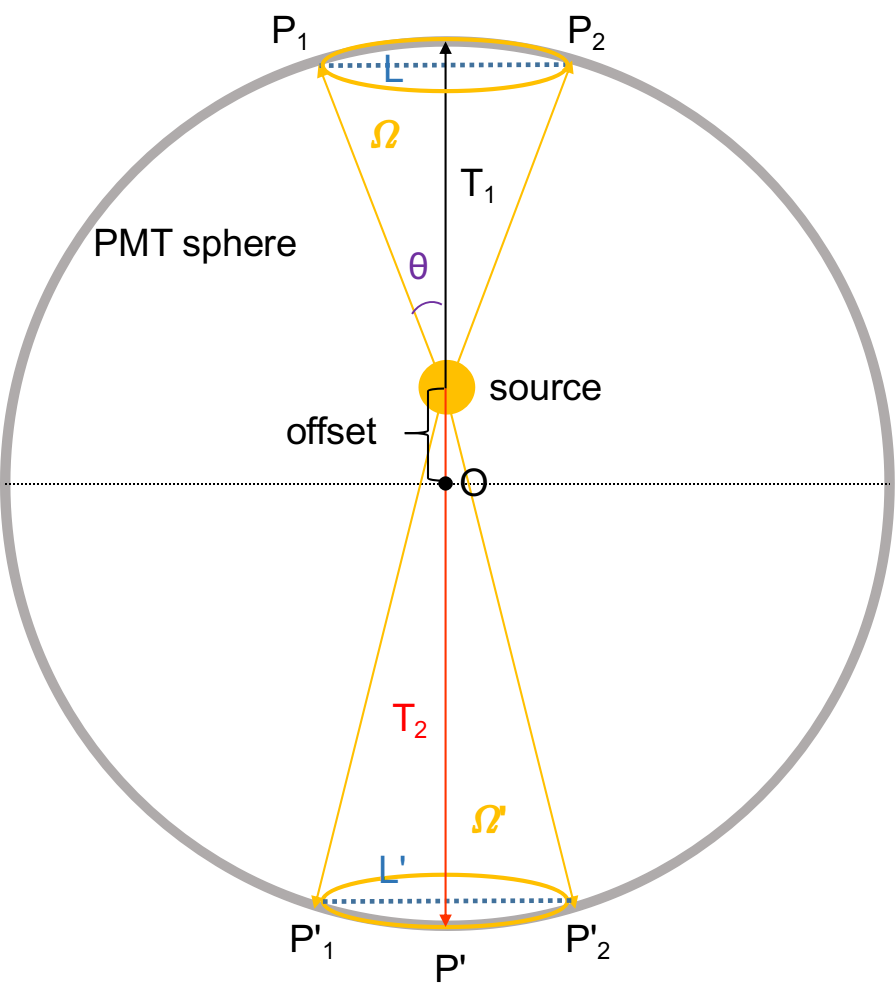
\includegraphics[width=6cm]{n16_groupVelocity.png}
	\caption{$^{16}$N central run.}
	\label{n16_groupVeloctiy}
\end{figure}

For a more precise approach, a set of laserball calibration runs which  to measure actual group velocities in the SNO+ water detector\cite{groupVmeasure}. 
 
For the scintillator and partial-fill phase vertex fitters, I adopt a linear interpolation method described in \cite{coulter2013modelling}, which will be discussed in section \ref{scintFitter}.

\subsection{Fitter Pull and Drive Correction}

An effect of ``fitter pull'' in the event vertex reconstruction utilizing the Cherenkov light was observed in the SNO experiment. The distribution of $(\vec{x}_{fit}-\vec{x}_mc)/|\vec{x}_{fit}-\vec{x}_mc|\cdot \vec{u}$ shows a large peak at +1, which indicates that the fitted position $\vec{x}$ is prone to be pulled forward from the true position systematically along the event direction$\vec{u}$\cite{driveCorPeter,brice1996monte,coulter2013modelling}. 

In the SNO+ water detection medium (or the SNO heavy water), Cherenkov photons created by an event trigger most of the PMT-hits with early timing and these hits are located within the Cherenkov cone; for the same event, there are also a few PMT-hits with later timing. These PMT hits can be caused by the scattered or reflected photons and they are located throughout the detector. For a random PMT hit, it is more probable to be placed outside the Cherenkov cone due to the geometry: consider an event happens at the center of the PSUP, the Cherenkov cone it produced will intersect the PSUP by an area of $2\pi R^2_{PSUP}(1-\cos41^\circ)$, which occupies about 12\% of the total area of the PSUP sphere. Therefore, for a random PMT-hit on the PSUP sphere, it has more than 88\% of chance to be placed outside the Cherenkov cone. 

For these later timing PMT hits, a similar ``complementary'' effect mentioned in \ref{tuneGroupVelocity} can also happen. When the fitter fits with $t_{res}$, for the large $t_{res}$ values caused by the later timing hits, it pulls the trial position away from the later timing hits to increase $t_{transit}$ and decrease $t_{res}$, as illustrated in Fig.~\ref{fitterPull}. This effect was also explained as ``straighten out delayed photons'' by the timing fitter in \cite{driveCorPeter}. Furthermore, the major early hits can also cause small $t_{res}$ values and thus the fitter pulls the trial position closer towards the early hits to decrease $t_{transit}$ and increase $t_{res}$. Recall that the early hits are located on or around the Cherenkov cone, therefore an overall effect of this ``fitter pull'' is that the fitted position will be pulled along the axis of the Cherenkov cone and towards the PSUP sphere. This pull direction is coincident with the event direction.

\begin{figure}[!htb]
	\centering
	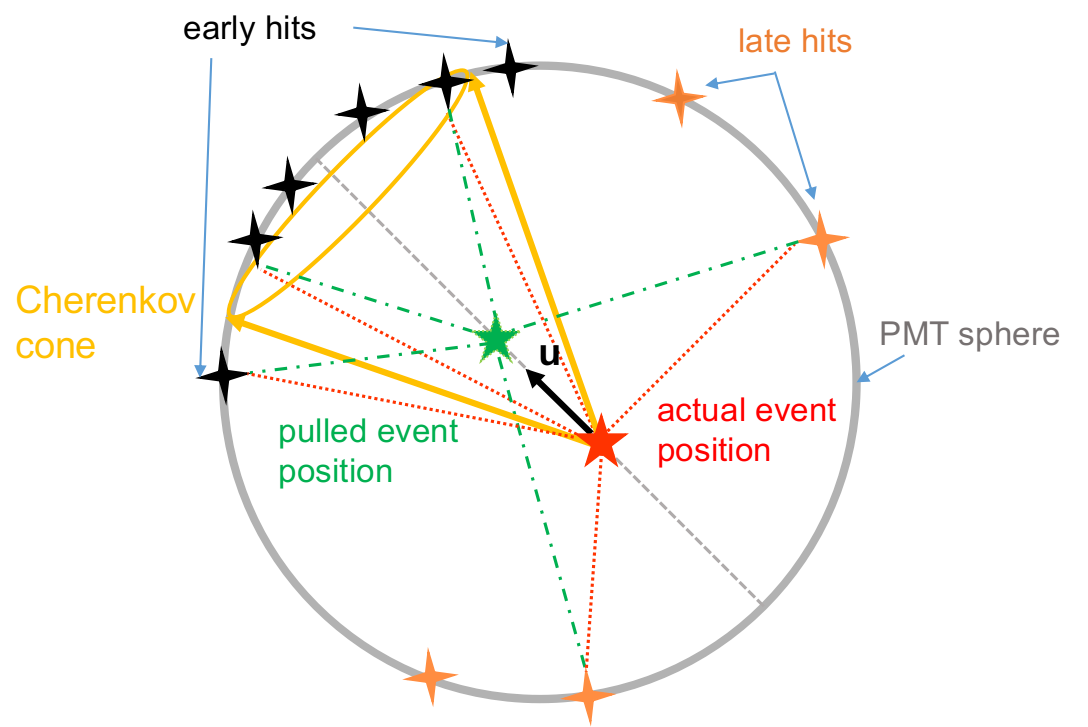
\includegraphics[width=8cm]{fitterPull.png}
\caption{ A cartoon shows fitter pull effect, modified from Fig.~C.2 in \cite{brice1996monte} and Fig.~2,3,4 in \cite{driveCorPeter}.}
	\label{fitterPull}
\end{figure}

A simple way to eliminate this ``fitter pull'' effect is to pull back the fitted event position against the event direction. This is called ``drive correction''.   

Once the MPW fitter obtains both of the fitted position and direction, the drive correction is applied on the fitted position by $\vec{X}_{\mathrm{corrected}} = p_0\vec{X}_{fit}+p_1\vec{u}_{fit}$, where $p_0$ and $p_1$ are the correction parameters, as shown in Fig.~\ref{drivecor}.
\begin{figure}[!htb]
	\centering
	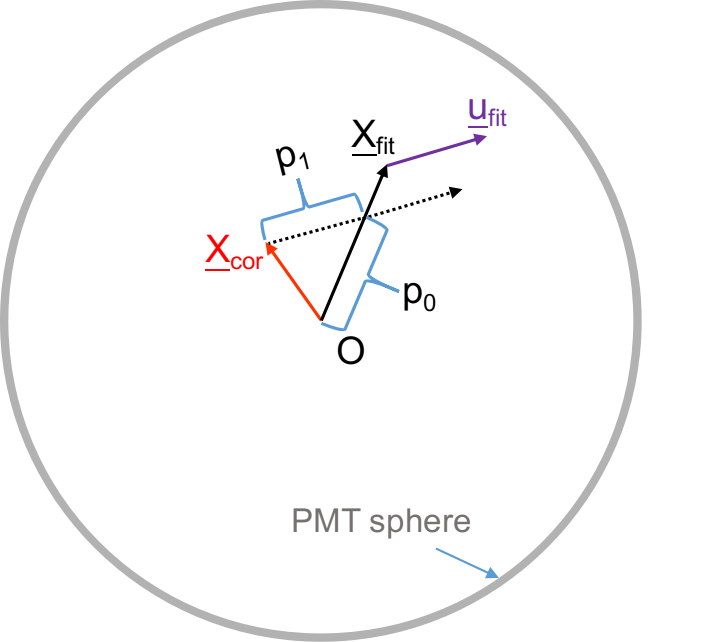
\includegraphics[width=6cm]{driveCor.png}
	\caption{ A diagram illustrates the drive correction.}
	\label{drivecor}
\end{figure}

To obtain the values of $p_0$ and $p_1$, I generated electron events distributed isotropically inside the AV. The simulations of 2, 3, 4, ... ,10 MeV electrons are produced. Then the MPW fitter is applied on each simulations and returns the results of $\vec{X}_{fit}$ and $\vec{u}_{fit}$. Take the Monte Carlo generated positions $\vec{X}_{MC}$ as the true positions, for all the fitted events, a $\chi^2$ function is calculated by:
\[
\chi^2 = \sum_{i=1}^{N_{\mathrm{events}}}[\vec{X}^i_{MC}-(p_0\vec{X}^i_{fit}+p_1\vec{u}^i_{fit})]^2
\]

The $p_0$ and $p_1$ are obtained by minimizing the $\chi^2$ function. When calculating the $\chi^2$, the fitted events of $|\vec{X}_{fit}-\vec{X}_{MC}|>3~m$ are thrown away to improve the $\chi^2$ minimization results.

For the 2 to 10 MeV electrons simulations, the obtained values of $p_0$ and $p_1$ are energy or Nhit dependent. However, it does not improve the results if using the Nhit dependent functions $p_0(Nhit)$ and $p_1(Nhit)$ as drive corrections.
Finally we take the average values from the 5 to 10 MeV electrons simulations and the drive correction is set as $\vec{X}_{\mathrm{corrected}} = 0.995765\vec{X}_{fit}+-63.826\vec{u}_{fit}$.

It is important to note that since the drive correction parameters are obtained from the reconstructions of Monte Carlo, it depends on the Monte Carlo and the results of reconstruction. Therefore, the n$_{water}$, mode cut and time residue cut affecting the fitted results will also affect the drive correction parameters, but not significantly.


\begin{figure}[!htb]
	\centering
	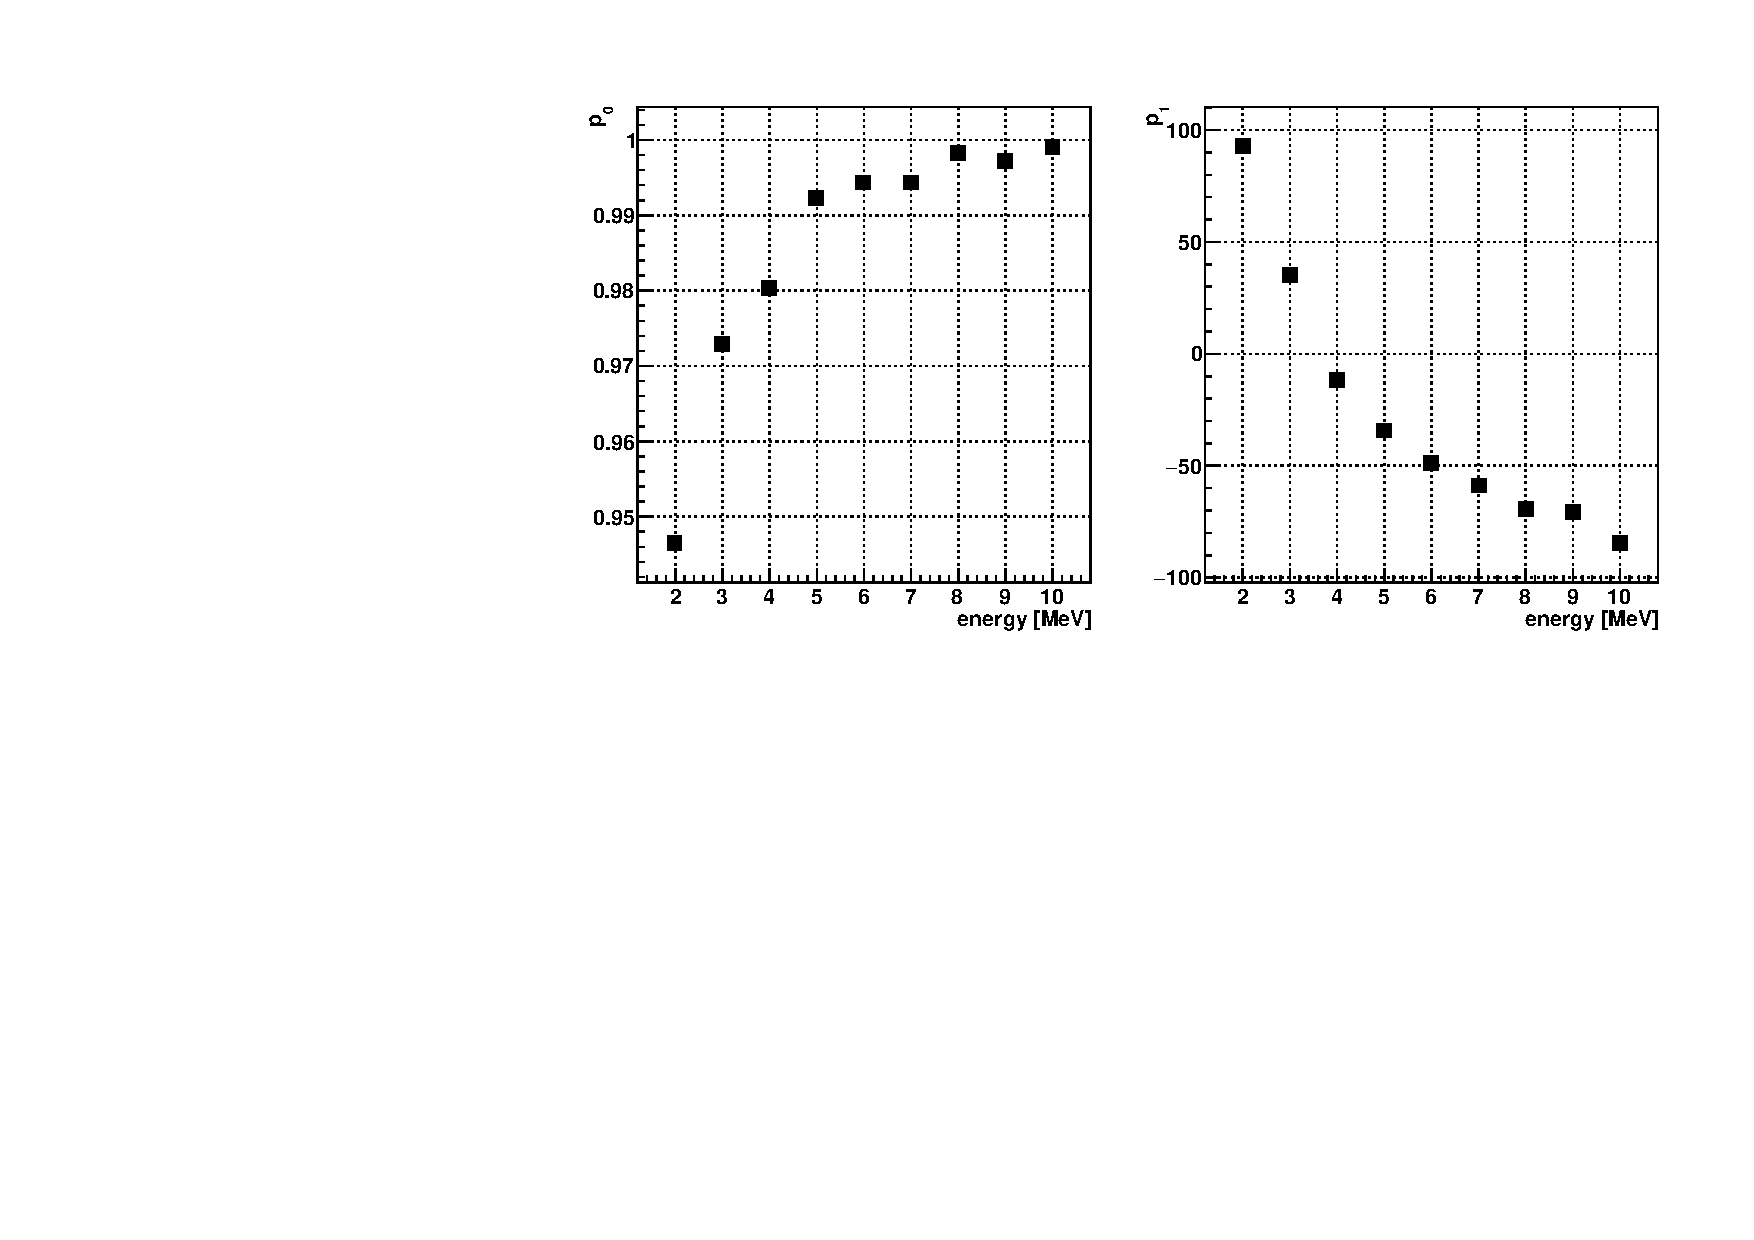
\includegraphics[width=10cm]{pullParVsEnergy.pdf}
	\caption{ Drive correction parameter $p_0$, $p_1$ vs energy.}
	\label{pullParVsEnergy}
\end{figure}

Electron events with various energies were generated at the detector center and their momentum were along +x direction. 

\begin{figure}[!htb]
	\centering
	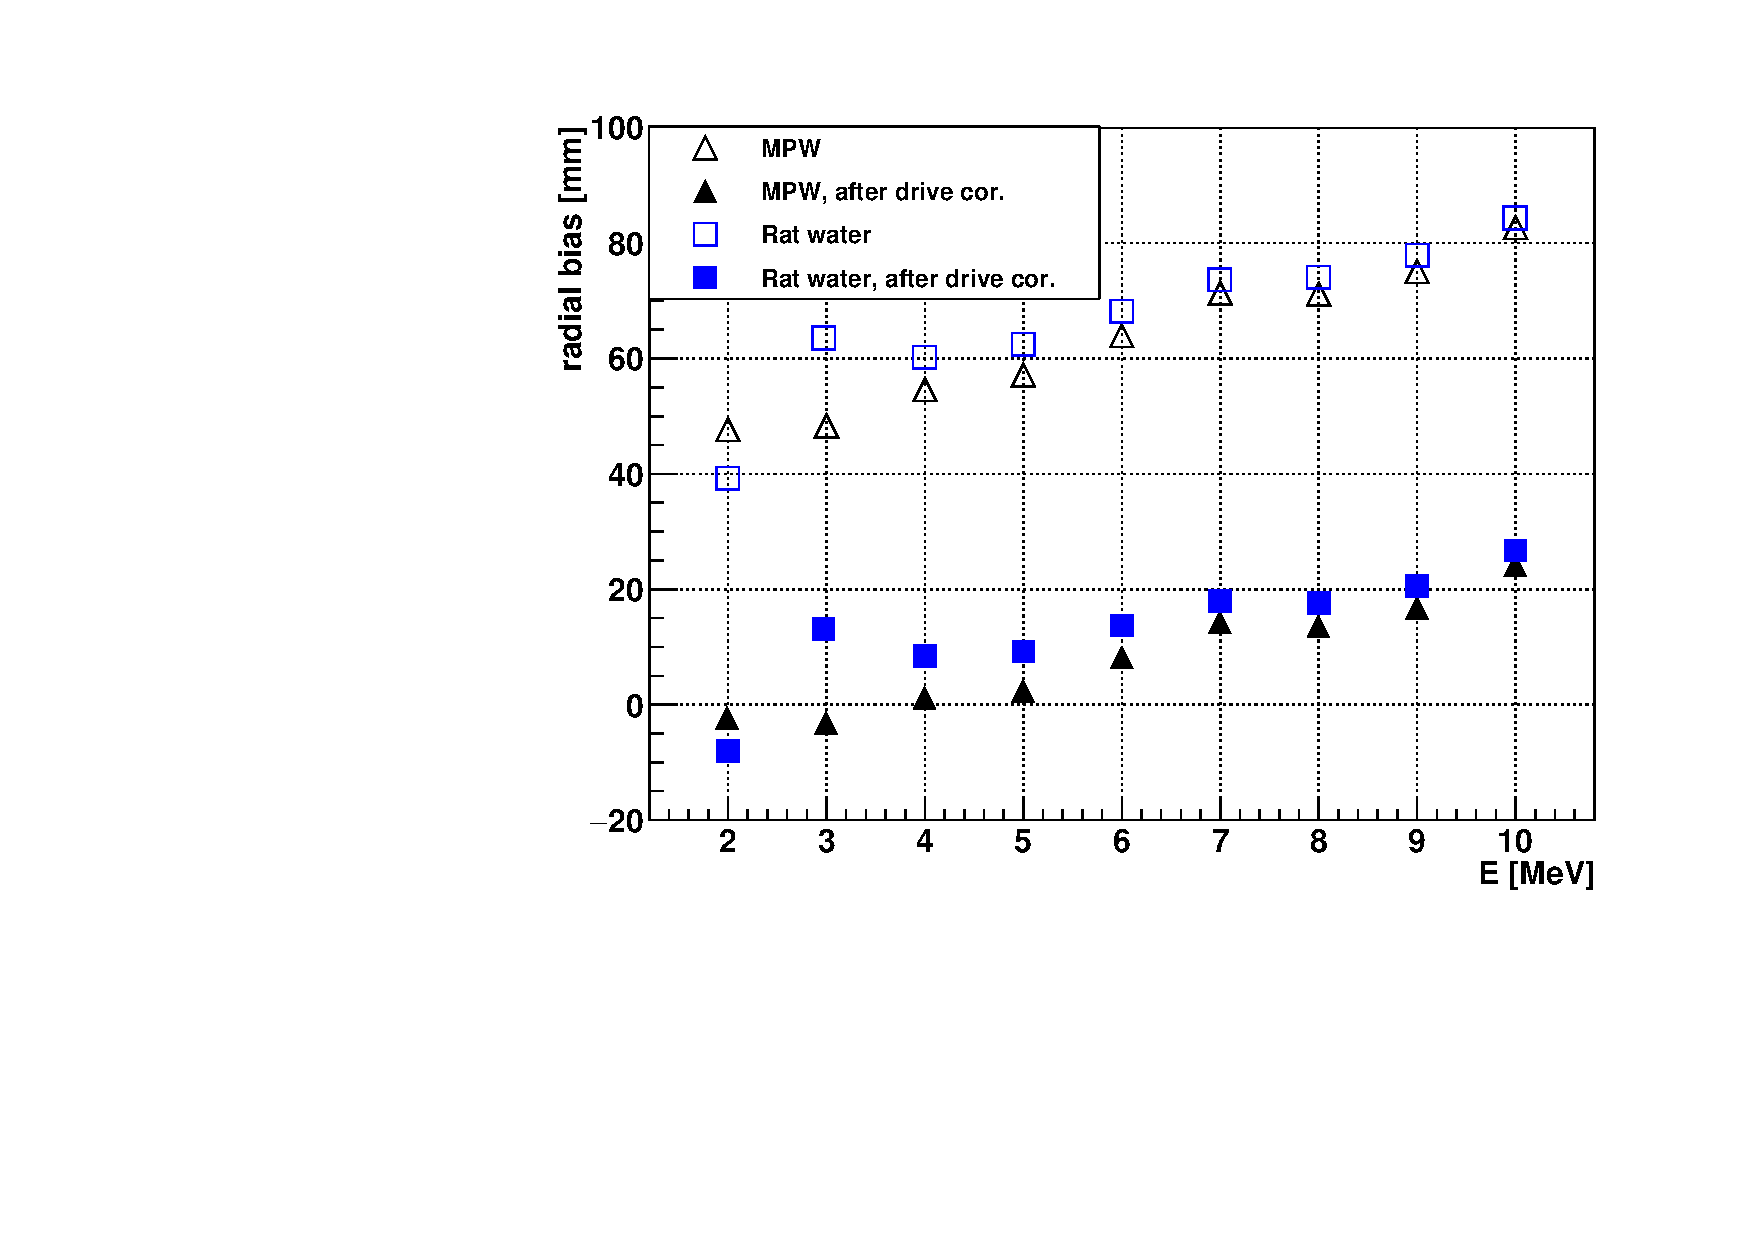
\includegraphics[width=8cm]{pullEffectVsEnergy.pdf}
	\caption{ Radial biases of simulated electron events before and after the drive correction, as a function of energy.}
	\label{drivecorVsEnergy}
\end{figure}


By fitting the simulations of 5 MeV electrons generated at the detector center and travelling along +x direction, the drive effct of the MPW fitter causes a $\sim$50 mm biases from the detector center along +x axis. The drive correction reduces this drive bias down to $\sim$0.2 mm. For the reconstruction of $^{16}$N data, the drive correction can reduce the fitted position RMS by $\sim$20 mm.

\subsection{Multi-path Fitter Structure}
The Multi-path fitter has already been implemented into the RAT software and being used in data processing and analyzing.

The MP fitter structure consists of: 
\begin{itemize}
\item[$\bullet$] Fitter database

This database provides parameters used by the fitter, including the physics constants, detector geometry parameters, fit parameters and pdfs. The database is in a JSON format\cite{JSONwiki} and contains multiple tables tagged by indices to indicate different detection media or physics phases. In each table, there are fit parameters and pdfs optimized for the specific scintillator. For example, for the partial-fill phase with a PPO concentration of 0.5 g/L, the fitter will look for the index of ``labppo\_0p5\_scintillator'' and extract the pdfs and fit parameters under that index.  

The fit parameters includes the fitter tolerance and the maximum iterations which determine how the fitter converges, 

Reflective index (water\_RI, or n$_{water}$), used for effective group velocity ($v_g$ =c/n$_{water}$) calculation. 
air refractive index (air\_RI), PSUP radius ($r_{PSUP}=8390~mm$). Offsets
boundary settings


The MPW fitter currently uses one fixed number for n$_{water}$, rather than a function of wavelengths. The value of n$_{water}$ can be tuned to give the lowest biases of the fitted positions to the Monte Carlo and to give the lowest RMS of fitted results as well. But the effect of n$_{water}$ can also be corrected by the drive correction afterwards. Currently n$_{water}=1.38486$ is obtained by analyzing the time of flight from the \isotope[16]{N} central run-100934 data reconstructed by the MPW fitter. 

time offset, position offset, radius cut x, fitting bin-width and steps.


- PMT response time (timing) pdf for the position reconstruction, as shown in Fig.~\ref{MPW_timingPDF}. The pdf shown in red line is modified from the measured PMT response time distribution from SNO time and the late light response is forced to be de-weighted (black). The pdf is modified in [-100,-4] ns region to match the time residual spectrum obtained from \isotope[16]{N} central run-100934 (blue).

- PMT angular response pdf for the direction reconstruction, as shown in Fig.~\ref{MPW_angularPDF}. It is taken from the Monte Carlo simulation of 5 MeV electrons traverse in the AV with one direction.


\item[$\bullet$]  Likelihood Calculation Classes, 
Constructs likelihood functions, calculates likelihoods and their derivatives. For the MPW fitter, there are two classes: WaterPosition for position reconstruction and \texttt{WaterDirection} for direction reconstruction. The \texttt{WaterPosition} class tackles with 4 parameters (x,y,z,t) and the \texttt{WaterDirection} class tackles with 2 parameters ($\theta$,$\phi$). 


\item[$\bullet$] Multi-path Fitter

Processes the MPW fitter and finds the best-fit of the likelihood function. It is a general processor and is shared with the fitters using the Multi-path Fitter, including the MPW fitter, air-water (AW) fitter, wavelength-shifter (WLS) fitter and scint-water fitter. It processes a certain fitter by being assigned the fitter name in macro. It processes the fitter event by event: for every triggered event, it first calls PMT selectors (ModeCut or StraightTimeResidualCut) and sends the information of the reduced PMTs to a certain Likelihood Calculation Class for likelihood calculations. The Likelihood Calculation Class sends back the values of likelihoods and their derivatives, so the Multi-path Fitter does not care about how the likelihood functions are constructed and how the likelihoods and derivatives are calculated. Using these values, it constructs an n$\times$n Hessian matrix (n is the number of fitting parameters defined in Likelihood Calculation Class) and uses the Levenberg-Marquardt (MRQ) method to maximize the likelihood and finds the best-fit values. For the MPW, if the likelihood maxima is found 5 times for any position and direction then values are returned as the fitted position and direction. For the MPW case, it calls the \texttt{ModeCut} and fits for the position and time; then it calls the StraightTimeResidualCut and fits for the directions.

\item[$\bullet$] \texttt{Dump Likelihood}

This is a function inside the Multi-path Fitter. It stores the likelihood surfaces and derivatives with respect to arrays of trial vertices of the interested events which are designated by event GTIDs in the database. From the likelihood surfaces and derivatives of an interested event, people can evaluate the fit performance of that event by checking whether the fitter finds global or local maximum. 

\item[$\bullet$] \texttt{SDecompQRH}

This s a fit method class modified from \texttt{ROOT TDecompQRH} class\cite{TDecompQRH}. It is used by the Multi-path fitter to invert the Hessian matrix through QR decomposition method\cite{press2007numerical}. Compared to ROOT, Solve() for Ax=b is modified to zero the component of x for which the diagonal element in R is small. This allows a Levenberg-Marquardt optimization to continue in many cases
when the matrix is singular. For the MPW case, it is used to invert a 4$\times$4 matrix of the WaterPosition Class while the inversion of 2$\times$2 matrix of the WaterDirection is calculated directly\cite{waterunidoc}.

\item[$\bullet$] PMT selectors

Detailed descriptions are shown in section \ref{sect:PMTselector}.

\end{itemize}

\section{Vertex and Direction Reconstruction for the Water-based Wavelength-shifter}
A reconstruction algorithm was developed to investigate the proposal for the water-based wavelength-shifter, as mentioned in \ref{sect:wbWLS}.

Figure~\ref{pmt_wls} shows the position distributions of hit PMTs for MC simulated 5 MeV electrons travelling along $+x$ direction in the AV. The left panel shows the case when the detector is filled with pure water while the right panel is for water plus 0.1 ppm PPO. For the same electrons, the number of hit PMTs ($NHit$) in wbWLS is about 2.4 times greater than the pure water one. Although there is extra isotropic light emitted, the Cherenkov ring can still be seen clearly, allowing reconstruction of the directionality.  

\begin{figure}[htbp]
	\centering
	\begin{minipage}[t]{0.48\textwidth}
		\centering
		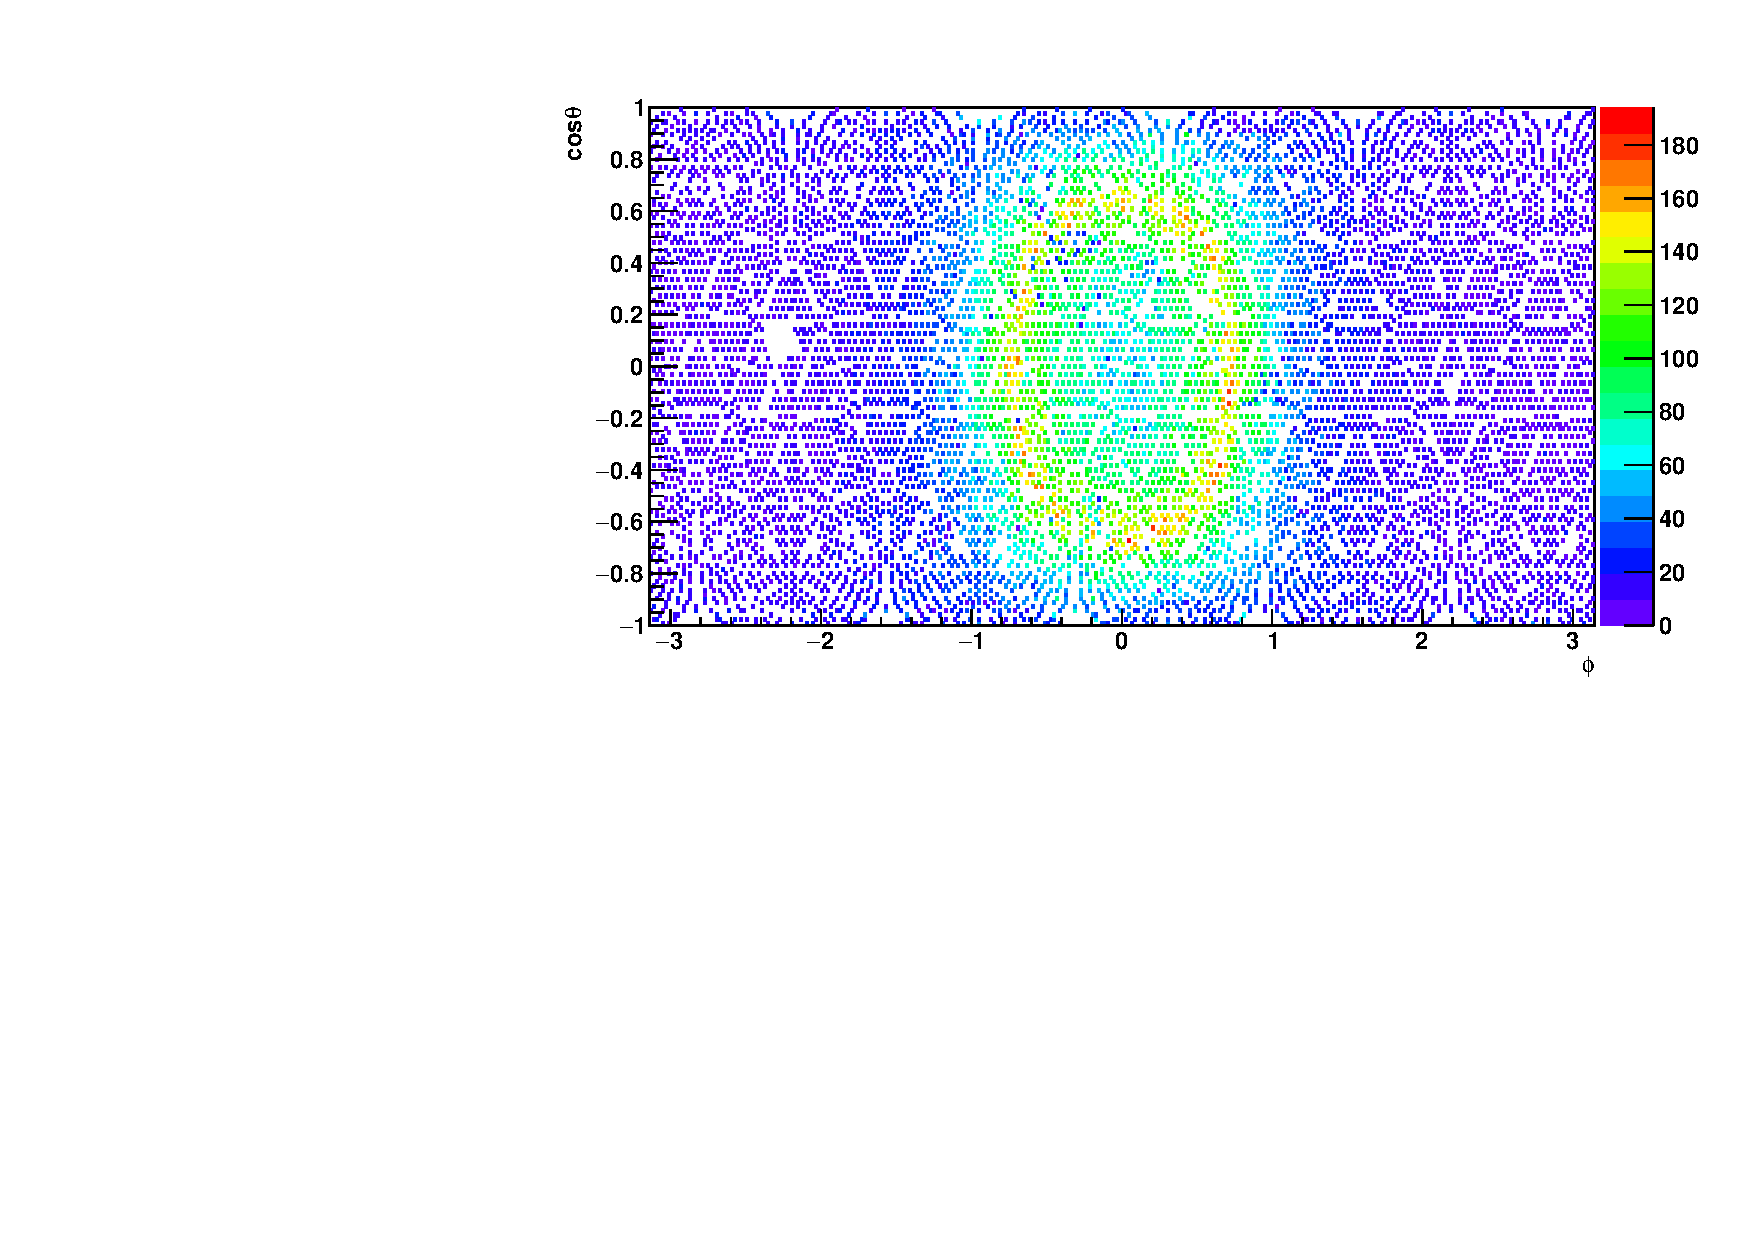
\includegraphics[width=7cm]{PMT_5MeVElectronWater.pdf}
	\end{minipage}
	\begin{minipage}[t]{0.48\textwidth}
		\centering
		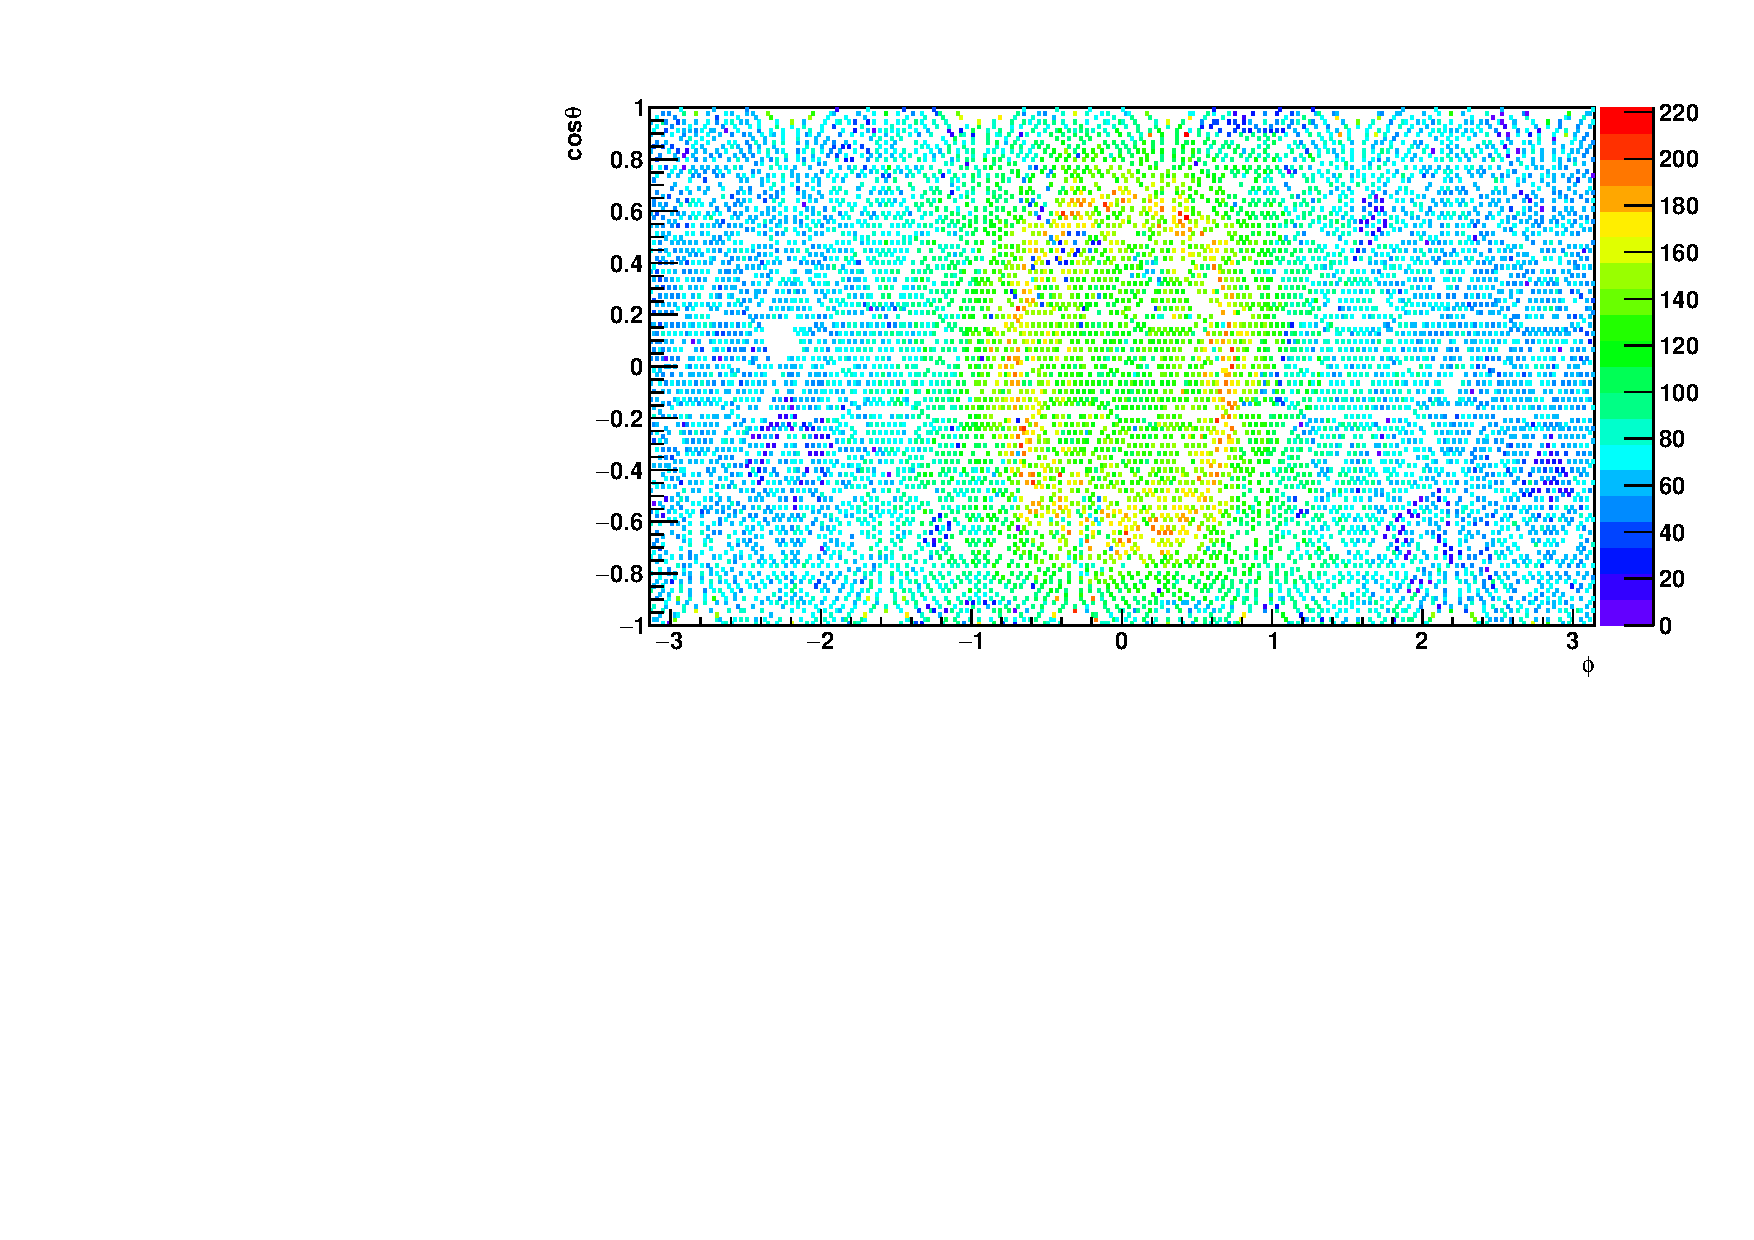
\includegraphics[width=7cm]{PMT_5MeVElectron0p1ppmPPO.pdf}
	\end{minipage}
	\caption{Position distributions of hit PMTs (in zenith and azimuth angles) for 5 MeV electrons travelling along $+x$ direction in the pure water (left) and the water plus 0.1 ppm PPO (right).}
	\label{pmt_wls}
\end{figure}

Figure~\ref{nhit_wls} shows the energies of simulated electrons as a function of the mean value of the $NHit$ distribution (mean nhits). In pure water, a 1 MeV electron simulation does not trigger any PMTs while in wbWLS case we have a mean nhits of 20.

\begin{figure}[htbp]
	\centering	
	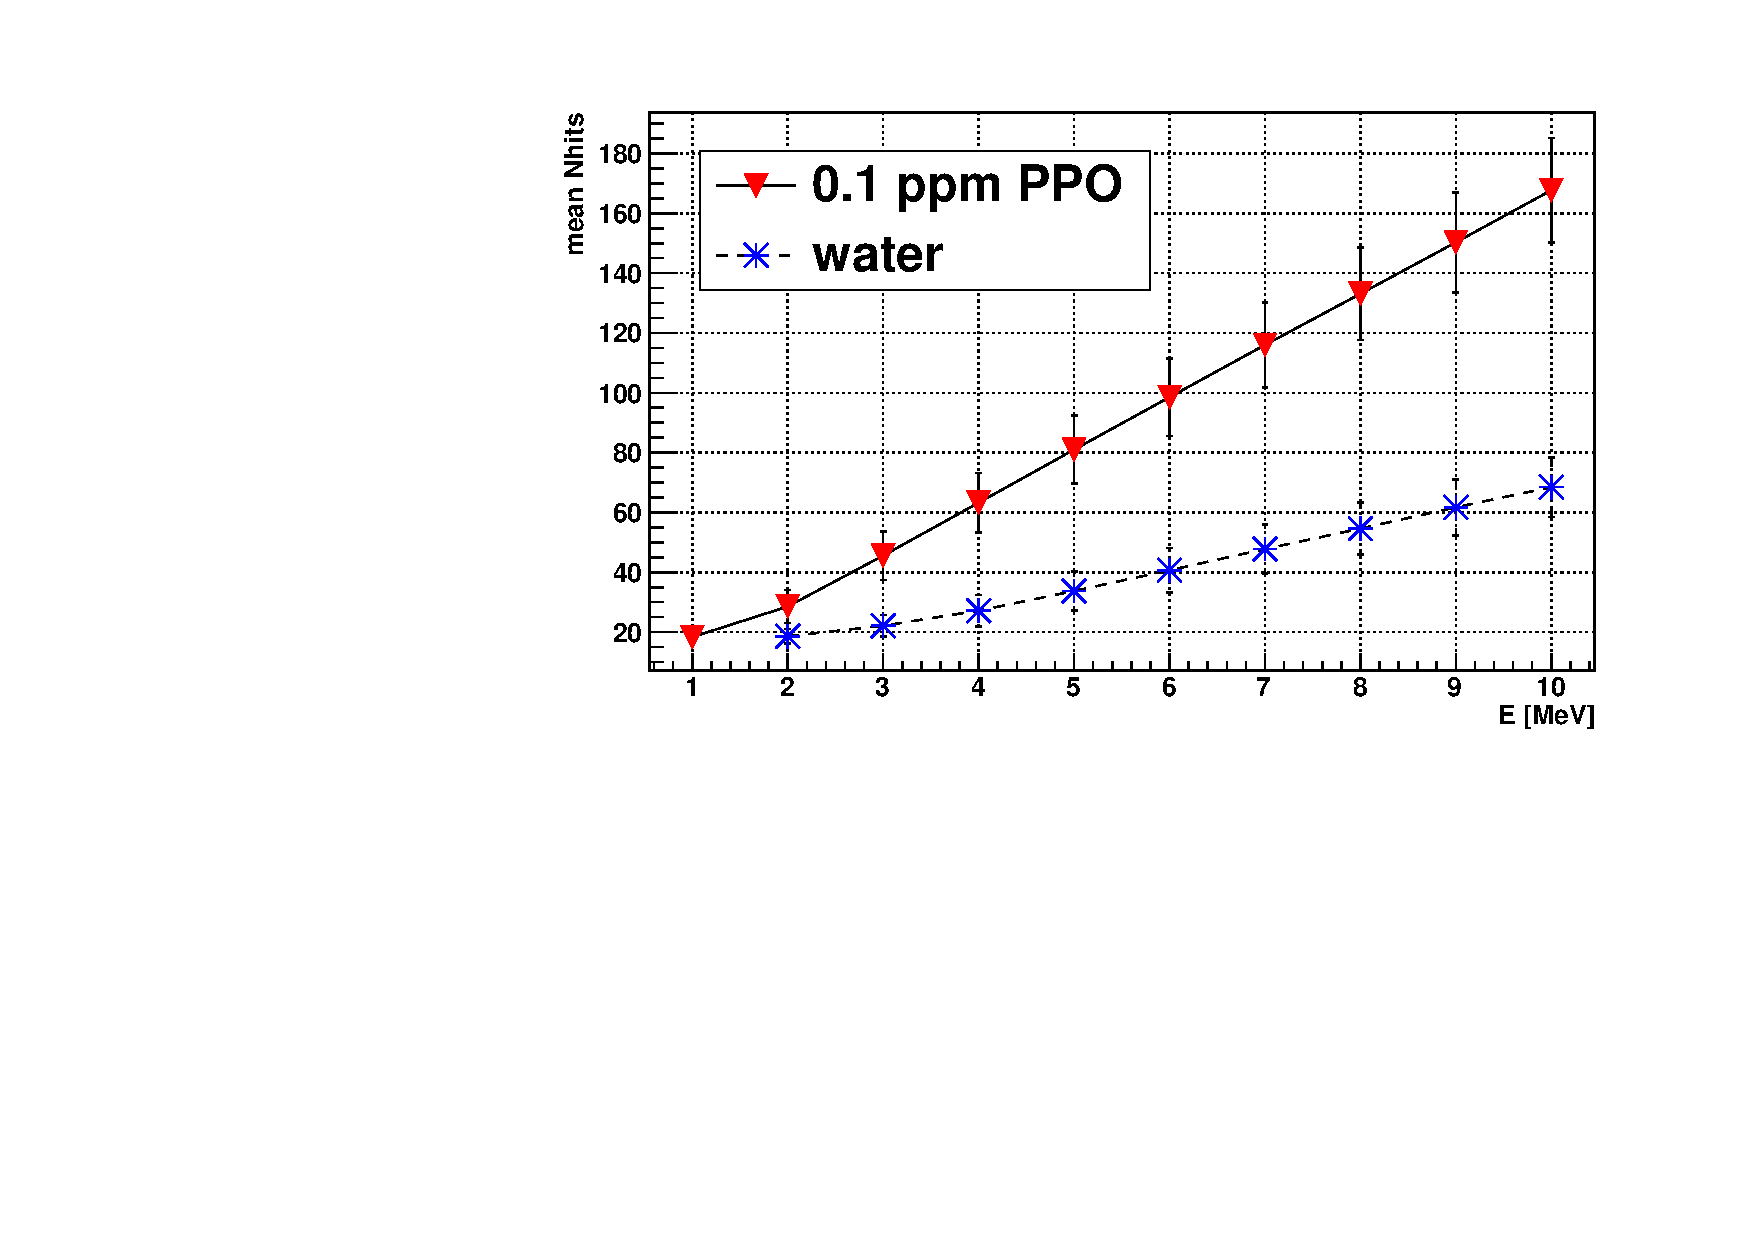
\includegraphics[width=9cm]{nhits_wls.pdf}
	\caption{ The energies of simulated electrons as a function of mean nhits. The values in the 0.1 ppm PPO (solid line with inverted triangle) are compared with the water (dashed line with star).}
	\label{nhit_wls}
\end{figure}

In the wbWLS case, since WLS absorbs and re-emits photons, the reconstruction mentioned in section \ref{sect:mpw} is slightly modified to build the MP WLS Fitter. According to the optical property of PPO, the prompt light emitted from an event has a probability of $\sim$0.6 to be absorbed by the WLS and then re-emitted at a shifted vertex along the particle direction $\hat{n}$. Then the fitter returns a shifted vertex, $\vec{X}_{0,shifted}=\vec{X}_0+\mathrm{offset}\cdot\hat{n}$. The offset we set in the fitter is 100 mm obtained from simulations. Figure~\ref{WLS_pdf} shows the timing pdf for the wbWLS, which is the PMT response time modified to photon propagation time in the wbWLS.
\begin{figure}[htbp]	
	\centering		
	\begin{minipage}[b]{0.5\textwidth}			
		%\centering			
		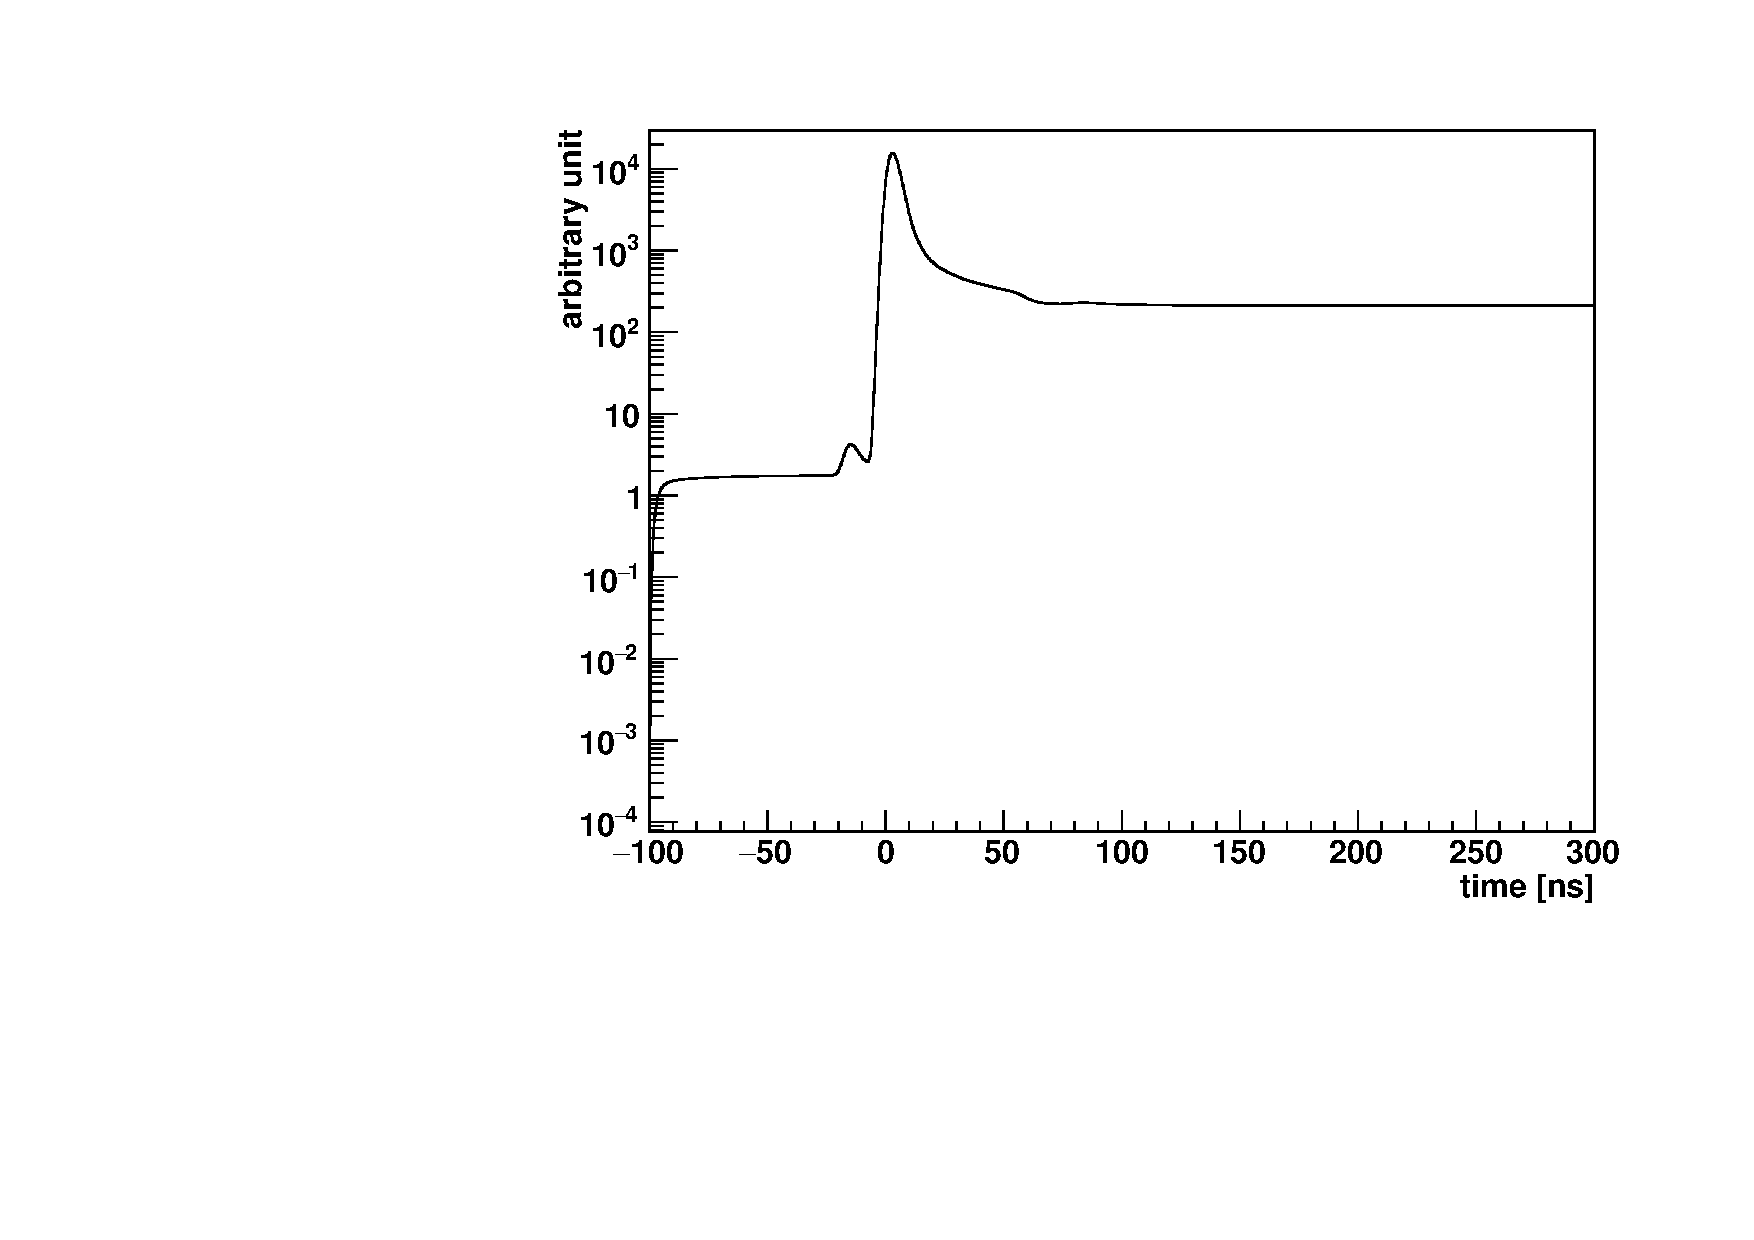
\includegraphics[height=6cm]{WLSTime_pdf.pdf}			
	\end{minipage}%				
%		\begin{minipage}[b]{0.5\textwidth}		
%			%\centering	
%			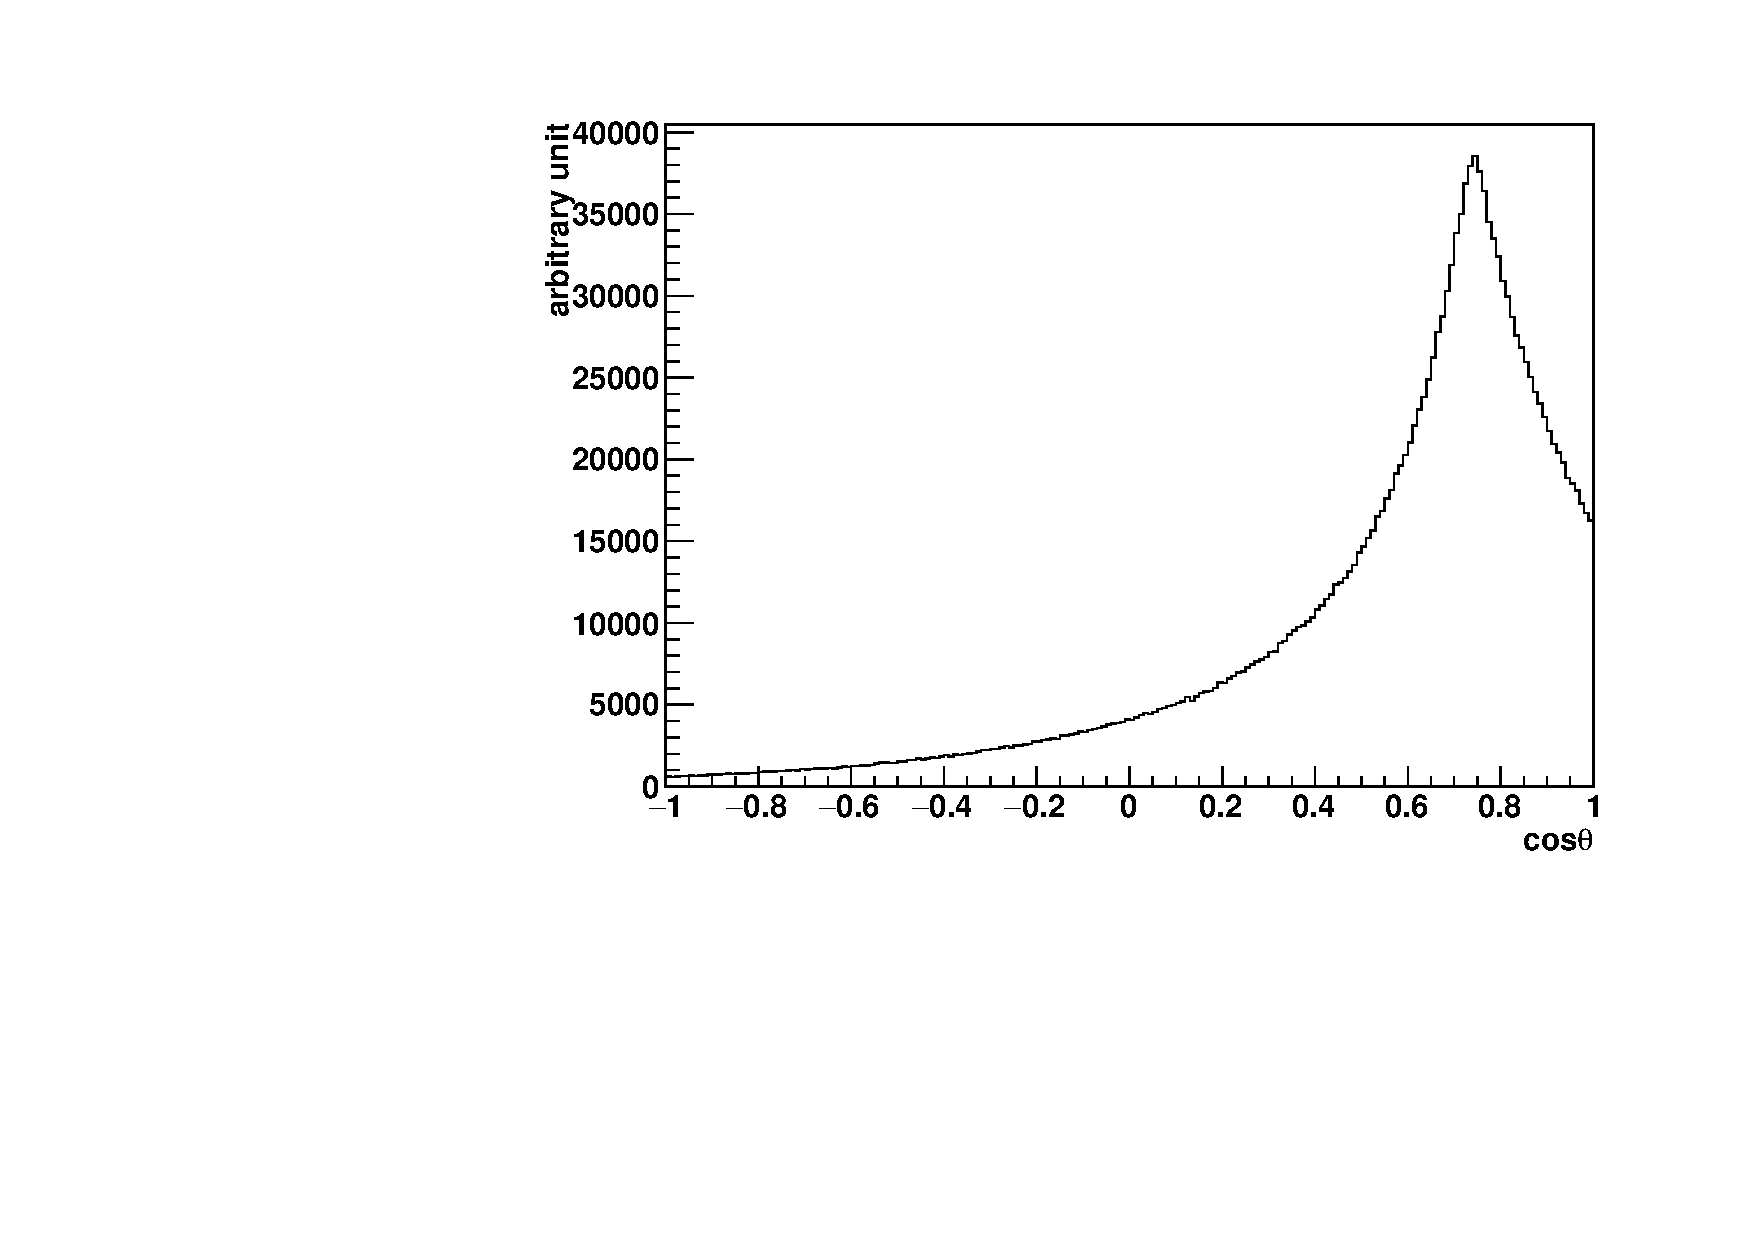
\includegraphics[height=5cm]{ChAngle_pdf.pdf}	
%		\end{minipage}	
	\caption{\label{WLS_pdf} The timing pdf for the wbWLS.}	
\end{figure}

To reconstruct the direction, besides the angular distribution of Cherenkov photons, $\cos\theta_{Ch}$, we also consider the fraction of the re-emitted and wavelength shifted photons that cause a flat angular distribution.

To test the performance of the MP WLS Fitter, 5 MeV electrons were simulated at the center of the AV filled with wbWLS and travelling along +x direction. As a comparison, the same simulation was done for the AV filled with pure water and the simulated events were reconstructed by the water fitter.

Fig.~\ref{WLSFitPos} shows the performance of the WLS fitter reconstructed positions of the MC simulations compared to the pure water case. For the fit position distribution of 5 MeV electrons in the wbWLS, we get a root mean square (RMS) of 201 mm and a bias to the center (the mean of histogram) of 29 mm. Compared to the pure water case, the fit bias is about 19 mm better and the RMS is 188 mm better.

\begin{figure}[htbp]	
	\centering			
	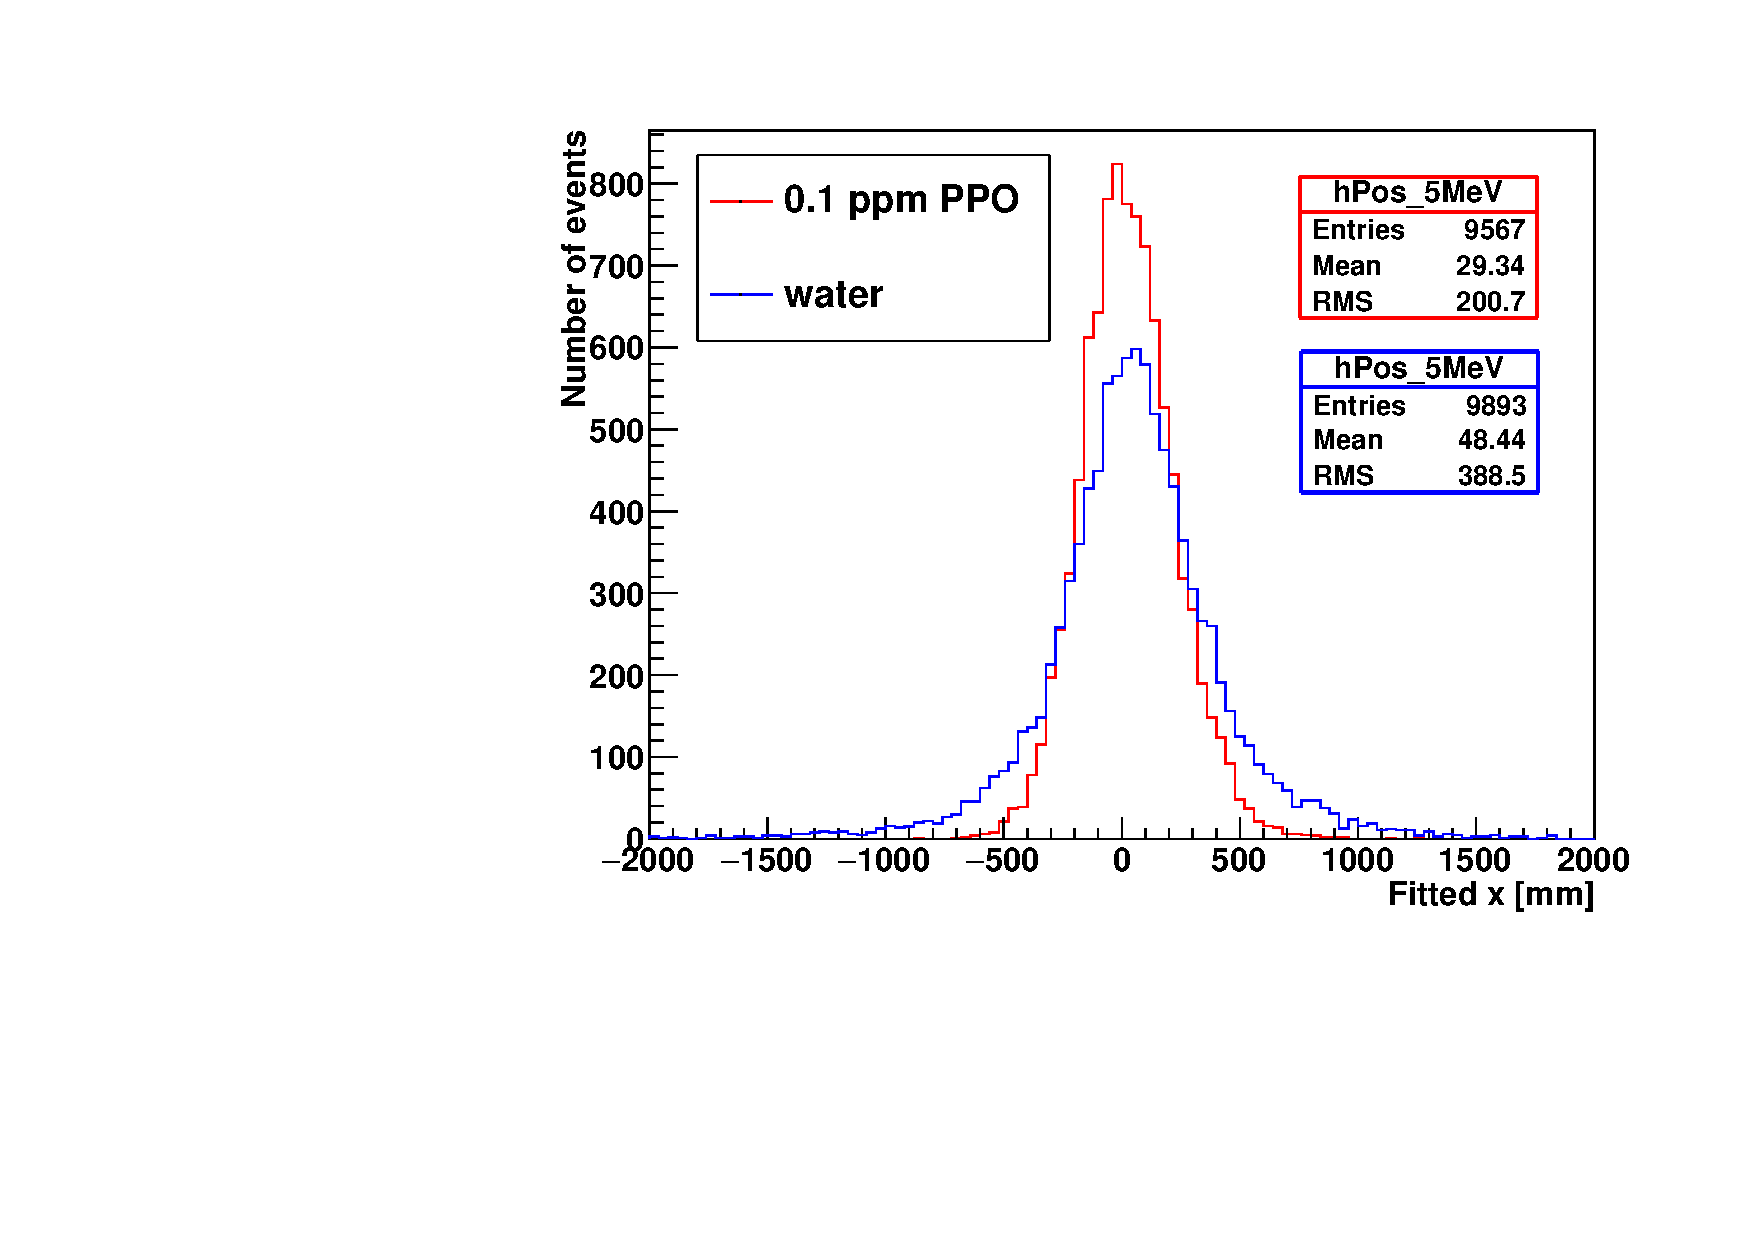
\includegraphics[height=5cm]{WLS_FittedPos.pdf}		
	\caption{\label{WLSFitPos} Fit position projected on x axis. The WLS fitter reconstructed $x$ positions of the 5 MeV electron events in the wbWLS (red) are compared to the ones in the water (blue).
	}
\end{figure}

For a given Cherenkov event, the error in the reconstructed event direction is defined as\cite{boulay2004direct}: $\cos(\theta_e)=\vec{u}_{fit}\cdot\vec{u}_e$, where $\vec{u}_e$ is the simulated electron direction and $\vec{u}_{fit}$ is the reconstructed direction. To quantify this error, we define a $\cos\theta_{a}$ so that:
\[
\frac{\int_{\cos\theta_{a}}^1 P(\cos\theta_e) d\cos\theta_e}{\int_0^1 P(\cos\theta_e) d\cos\theta_e} = a.
\] 
where $P(\cos\theta_e)$ is the distribution of $\cos\theta_e$ from MC data. The value of $\cos\theta_{a}$ is found numerically to let $\cos\theta_e$ contain $ a\cdot 100\%$ of the reconstructed data. A larger $\cos\theta_{a}$ means better direction reconstruction.

Table~\ref{quantAngular} shows the results of $\cos\theta_{a}$ for SNO heavy water data\cite{boulay2004direct} and simulations for SNO+ pure water and wbWLS. 

\begin{table}[ht]
	\caption{A comparison of quantitative estimates for the angular resolution between the SNO heavy water, SNO+ wbWLS and the SNO+ pure water cases.}\label{quantAngular}
				\centering		
		\begin{tabular*}{120mm}{c@{\extracolsep{\fill}}cccc}
			\toprule 
			medium & $\cos\theta_{0.9}$ & $\cos\theta_{0.8}$ & $\cos\theta_{0.5}$
			\\
			\midrule
			SNO heavy water  & 0.50 & 0.71 & 0.92  \\	
			SNO+ water  & 0.53 & 0.76 & 0.93	 \\
			wbWLS  & 0.37 & 0.63 & 0.90  \\	
			\bottomrule	
		\end{tabular*}
\end{table}

Comparing a pure water SNO+ detector and the wbWLS one, using the MP WLS Fitter for physics events gives a better position resolution without a significant loss in the performance of the direction reconstruction.

This fitter was tested for in \cite{mekarski2018electron}.

\section{Vertex Reconstruction for the Partial-fill and Scintillator Phases}\label{scintFitter}

In the partial fill geometry, photons will travel with different speeds as they pass through two different mediums, water and scintillator. Assuming a straight light path, the MP Partial Fitter mainly calculates the total length of the light path ($|\vec{l}_p|=|\vec{X}_\mathrm{PMT}-\vec{X}_0|$) and separates the $|\vec{l}_p|$ into the lengths in scintillator ($d_{sp}$) and in water ($|\vec{l}_p|-d_{sp}$).

\begin{figure}[!htb]
	\centering
	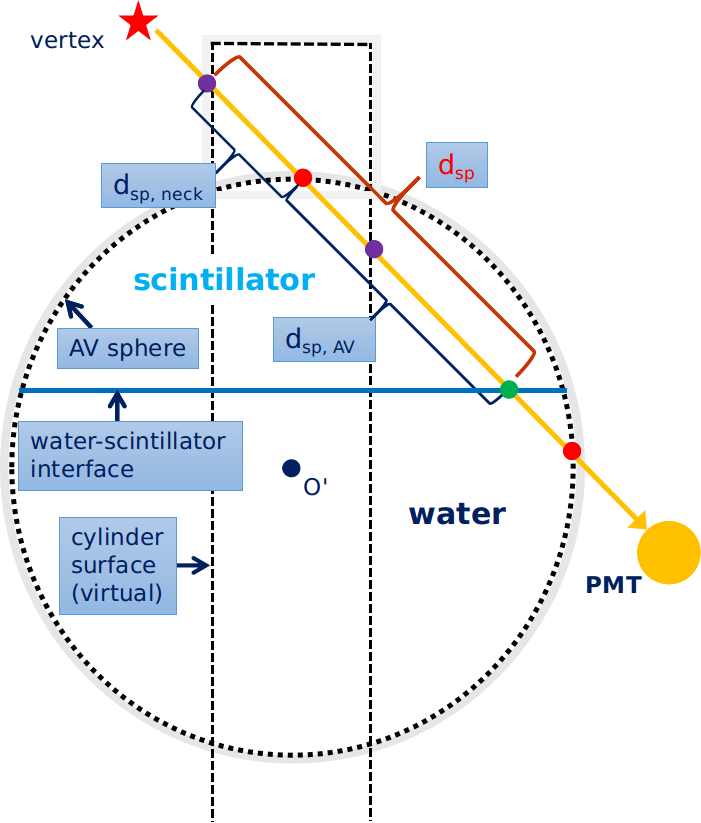
\includegraphics[width=7cm]{scintpath.png}
	\caption{Light path calculation for the MP Partial Fitter. The light path intersects with the neck cylinder surface, the AV sphere as well as the water-scintillator interface. The total length of the path in the scintillator region (scintillator path, sp), $d_{sp}$ is evaluated by intersection calculations.}
	\label{scintpath}
\end{figure}

In the partial-fill phase, the SNO+ detector can be considered as a geometry composed of the neck (cylinder), AV sphere and water-scintillator interface (plane). A ray connecting a position inside the PSUP to the PMT can intersect with these three geometries. As illustrated in Fig.~\ref{scintpath}, a detailed calculation of $d_{sp}$ includes evaluations of (1) light path and neck (ray-cylinder) intersection; (2) light path and AV sphere (ray-sphere) intersection and (3) light path and water-scintillator interface (ray-plane) intersection. $d_{sp}$ is further separated into the path length in the neck ($d_{sp,neck}$) and in the AV ($d_{sp,AV}$). 

For a trial position $\vec{X}_0=(x_0,y_0,z_0)$ and a hit PMT position $\vec{X}_{\mathrm{pmt}}=(x_\mathrm{pmt},y_\mathrm{pmt},z_\mathrm{pmt})$, define a light ray (rather than a line without direction) $\vec{l}_0\equiv\vec{X}_0+a\cdot \vec{u}$, where $a$ is the distance between vertex and intersection point and it is the parameter to be determined; $\vec u=\frac{\vec{X}_{\mathrm{pmt}}-\vec{X}_0}{|\vec{X}_{\mathrm{pmt}}-\vec{X}_0|}$ is the direction of the light ray. It is a unit vector pointing from the $\vec{X}_0$ to the $\vec{X}_{\mathrm{pmt}}$.

In the ray-sphere intersection case (light ray passes through the AV sphere), the intersection points on the $\vec{l}_0$ satisfy the sphere equation $(\vec{X}-\vec{O}_{av})^2= r^2_{av}$, where $\vec{O}_{av}$ is the origin of the AV sphere and $\vec{O}_{av} = (0,0,108)~mm$ in the PSUP coordinate. Thus the intersection equation is:
$(\vec{l}_0-\vec{O}_{av})^2 = r^2_{av}$.

Let $\Delta \equiv {[(\vec{X}_0-\vec{O}_{av})\cdot\vec{u}]}^2-{(\vec{X}_0-\vec{O}_{av})}^2+r^2_{av}$, if $\Delta>0$, solve the equation and get:
\begin{equation}\label{eq:ray-sphere}
a_{+,-} = -(\vec{X}_0-\vec{O}_{av})\cdot\vec{u}\pm\sqrt{\Delta},~if~\Delta>0.
\end{equation}
In this case, both $a_+$ and $a_-$ exist and have different values. If $a_+>a_->0$, the length of the path inside the sphere is $a_+-a_-$, as illustrated in Fig.~\ref{line-sphere} (a). Due to this geometry, the event position should be outside the AV, the condition $|\vec{X}_0|\geq r_{AV}$ is automatically met. If $a_+>0>a_-$, $a_-$ determines the intersection point along the opposite direction of the light ray. Thus the light ray actually does not pass that point (different to the line intersection with no direction). Thus the length of the path inside the sphere is $a_+$, as illustrated in Fig.~\ref{line-sphere} (b). Also, the condition $|\vec{X}_0|<r_{AV}$ is automatically met. 

If $\Delta\leq0$,
there is no intersection point or only one intersection point at the AV, the light ray never passes through the AV sphere, as illustrated in Fig.~\ref{line-sphere} (c) and (d).

\begin{figure}
	\centering
{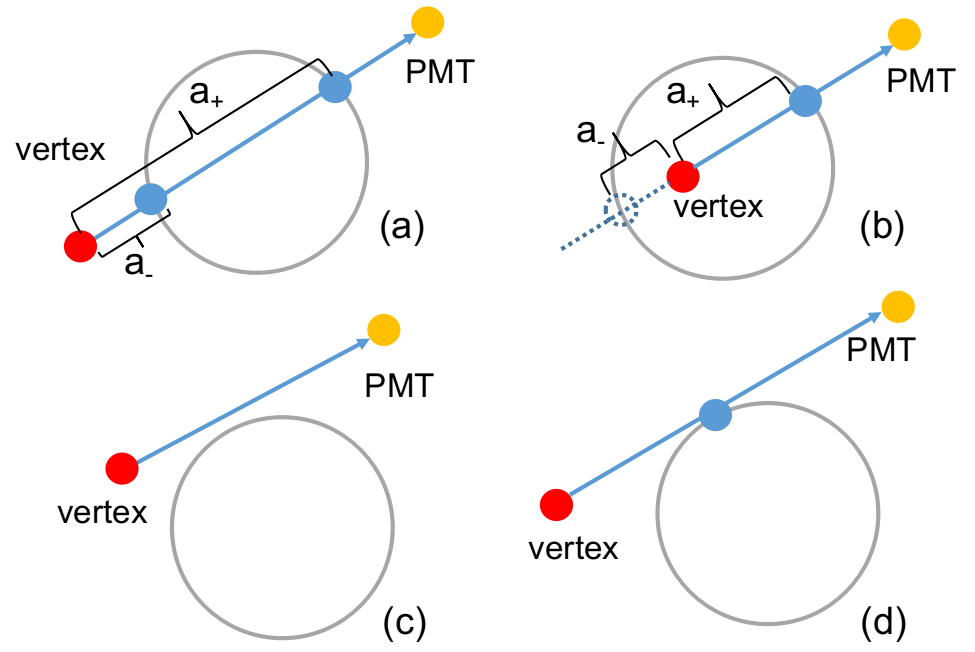
\includegraphics[width=80mm]{line-sphere.png}}
\caption{Line-sphere intersections. (a): the light ray intersects the sphere with 2 points; (b): the light ray intersects the sphere with 1 point; (c) and (d): the light ray never passes through the sphere.}\label{line-sphere}
\end{figure}

For the ray-plane intersection, the z components of the intersection points on $\vec{l}_0$ satisfy the plane equation $z=Z_{split}$, where $Z_{split}$ is the water level, i.e., the z position of the water-scintillator intersection. Thus the intersection equation is:
$l_{0,z}=Z_{split}$, where $l_{0,z}=z_0+a\cdot u_z$.

If $u_z=z_\mathrm{pmt}-z_0=0$, the ray is parallel to the plane and never intersects the plane.

If $u_z\neq 0$, solve the equation, we have: $a=(Z_{split}-z_0)/u_z=(Z_{split}-z_0)$.
Let: 
\[
a_3 \equiv a = \frac{(Z_{split}-z_0)|\vec{X}_{\mathrm{pmt}}-\vec{X_0}|}{z_\mathrm{pmt}-z_0}~~(if ~z_\mathrm{pmt}-z_0\neq 0).
\]

Similar to the case of ray-sphere intersection, if $a_3<0$, the ray-plane intersection point is on the extended line along the opposite direction to the ray; $a_3 \geq 0$ ensures the ray hits the interface. Note that here we consider the plane is infinitely large. Later we will combine with the calculations of the other geometries to cut it off. 

For the ray-cylinder intersection, the x and y components of the intersection points on the $\vec l_0$ satisfy the intersection equation: $l^2_{0,x}+l^2_{0,y} = r^2_{neck}$, where $r_{neck}$ is the radius of the neck cylinder ($r_{neck}=785~mm$).

To solve the equation,  let: $\Delta'\equiv [x_0\cdot (x_{PMT}-x_0)+y_0\cdot(y_{PMT}-y_0)]^2 - ( x_0^2+y_0^2-r^2_{neck})\cdot [(x_{PMT}-x_0)^2+(y_{PMT}-y_0)^2]$, and then we get: 
\begin{equation}\label{eq:ray-cylinder}
a'_{\pm} = |\vec{X}_{PMT}-\vec{X}_0|\cdot\frac{-[x_0\cdot (x_{PMT}-x_0)+y_0\cdot(y_{PMT}-y_0)] \pm \sqrt\Delta' }{(x_{PMT}-x_0)^2+(y_{PMT}-y_0)^2},~if~\Delta'>0,
\end{equation}

Similar to the ray-sphere case, if $a'_{+}>a'_->0$, the length of the path inside the cylinder is $a'_+-a'_-$. Due to this geometry, the event position should be outside the cylinder, the condition $(x^2_0+y^2_0\geq r_{neck}$ is automatically met. If $a'_+>0>a'_-$, the event position should be inside the cylinder and the ray-vector intersects the cylinder with one point (while the other point is along the opposite direction). Thus the length of the path inside the cylinder is $a'_+$. If $\Delta'\leq0$, the light ray never passes through the neck cylinder. Also note that here we consider the cylinder is infinitely long. This will also be cut off by the combined calculations of the other geometries. In addition, since only the neck region inside the PSUP is valid for the fitter, we should also ensure $z<8390~mm$ (in PSUP coordination).

To evaluate the length of the light ray (light path) in the scintillator region ($d_{sp}$), the above three geometries needs to be combined carefully. The following two procedures go through all the possible situations. First combine the evaluations of the ray-sphere and the ray-plane intersections to calculate the light path in the AV scintillator region ($d_{sp,AV}$). Then combine the evaluations of the ray-sphere and the ray-cylinder intersections to calculate the light path in the neck scintillator region ($d_{sp,neck}$).

Since the valid fit requires the events inside the PSUP sphere, only the neck region inside the PSUP sphere (with $6108<z_{neck}<8390~mm$) needs to be considered. The neck path calculation is allowed to be turned off. Detailed calculations are listed in \ref{sect:lightpath}.

Once the total lengths of the light path in the scintillator region or the water region are calculated, the time of flight, $t_{transit}$ is obtained by:
\begin{equation}
t_{transit} = \frac{|\vec{l}_p|-d_{sp}}{v_{gr,water}} +\frac{d_{sp}}{v_{gr,scint}},
\end{equation}
and thus the time residual, $t_{res}$ is calculated.

\begin{figure}[htbp]
	\centering	
	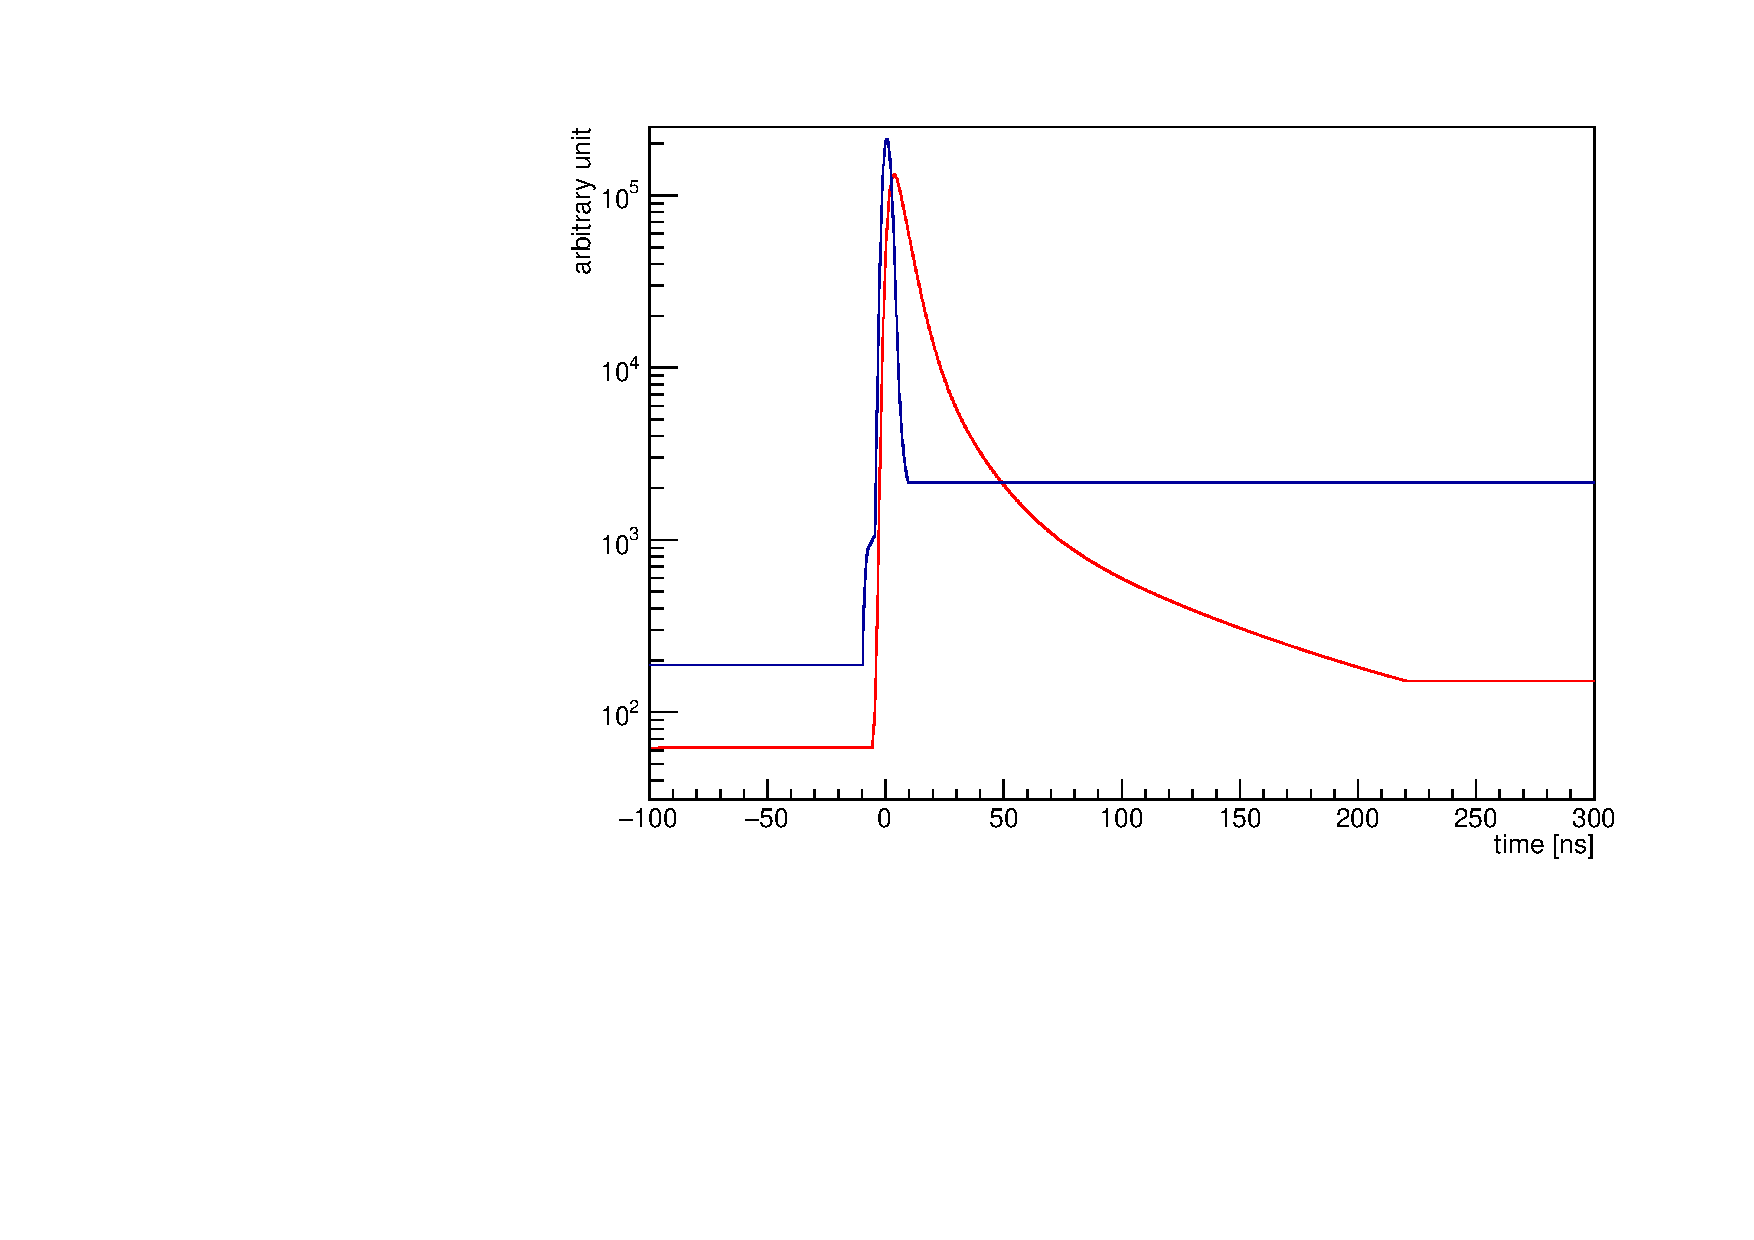
\includegraphics[width=7cm]{scintpdf.pdf}
	\caption{The timing pdfs used by the MP Partial Fitter. Blue: the timing pdf used by the MP Water Fitter; red: the scintillator timing pdf.}
	\label{partialpdf}
\end{figure}

If $d_{sp}=0$, the light path is always in the water. In this case, the fitter is the same as the MP Water Fitter. The fitter fits with the MP Water Fitter pdf. Once the light path passes through the scintillator region, the fitter fits with a scintillator timing pdf, the PMT time response modified to photon propagation time in scintillator, as shown in Fig.~\ref{partialpdf}.

\begin{figure}[htbp]
	\centering
	\subfigure[scintillator region]{
		\begin{minipage}[t]{0.38\textwidth}
			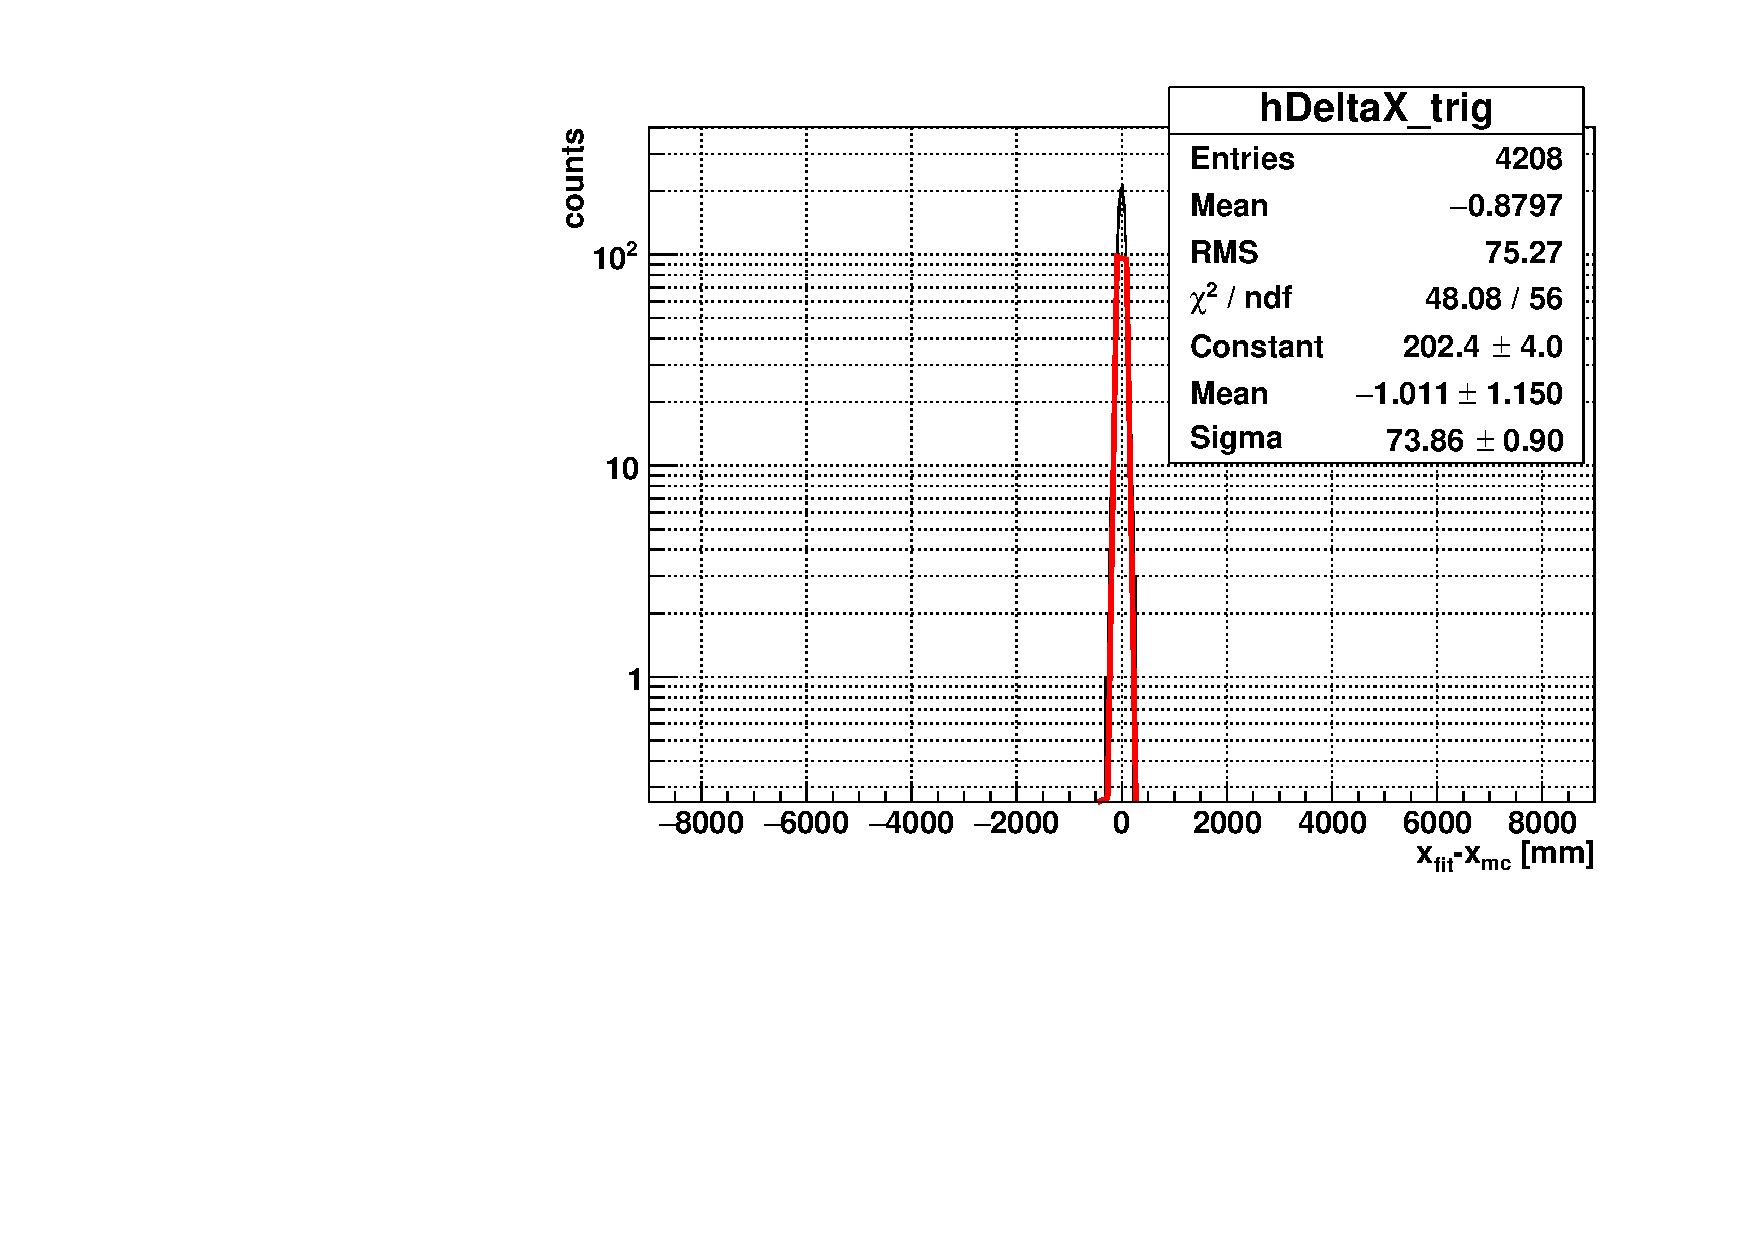
\includegraphics[width=6cm]{partial_top_x.pdf}
		\end{minipage}
	}   
\subfigure[water region]{ 
		\begin{minipage}[t]{0.38\textwidth}
			\centering
			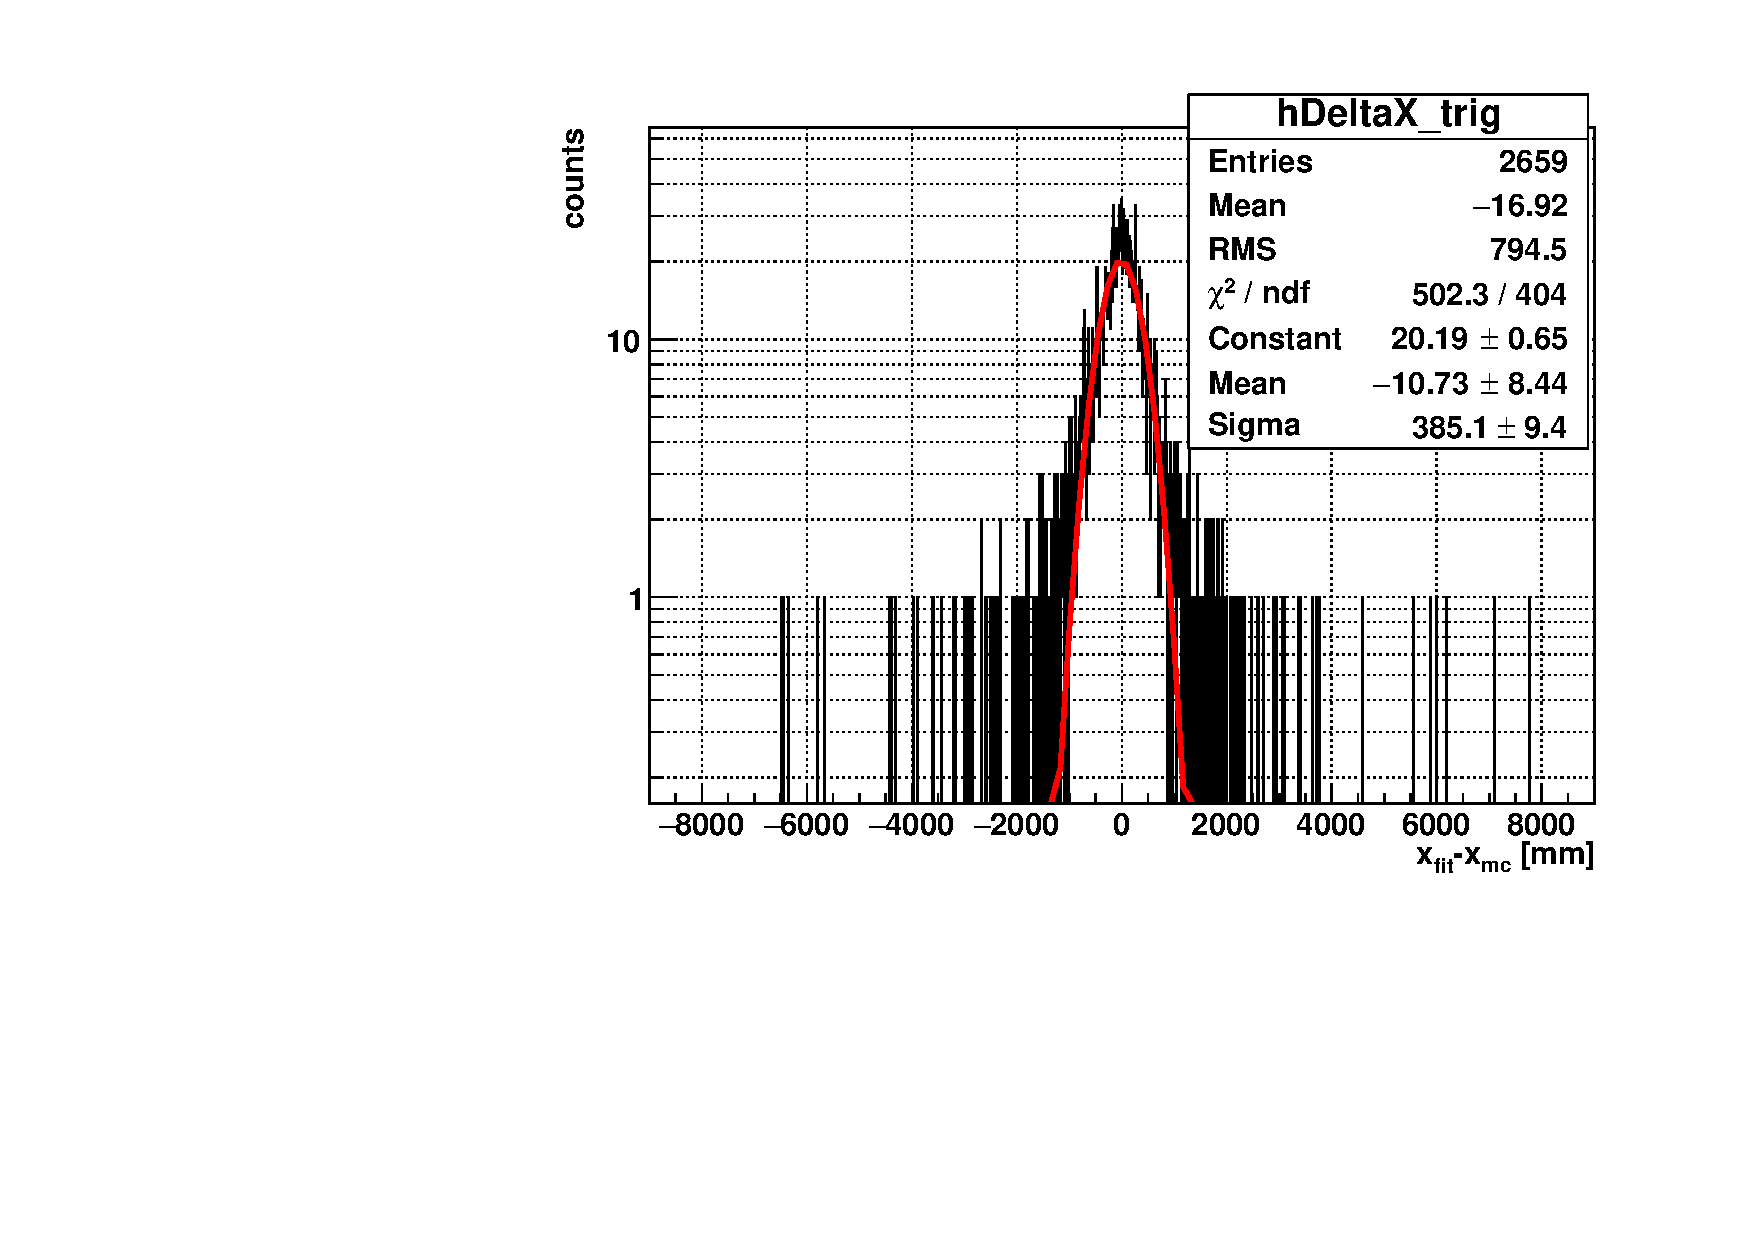
\includegraphics[width=6cm]{partial_bot_x.pdf}
		\end{minipage}
	}
	\subfigure[whole region]{ 
		\begin{minipage}[b]{0.32\textwidth}
			\centering
			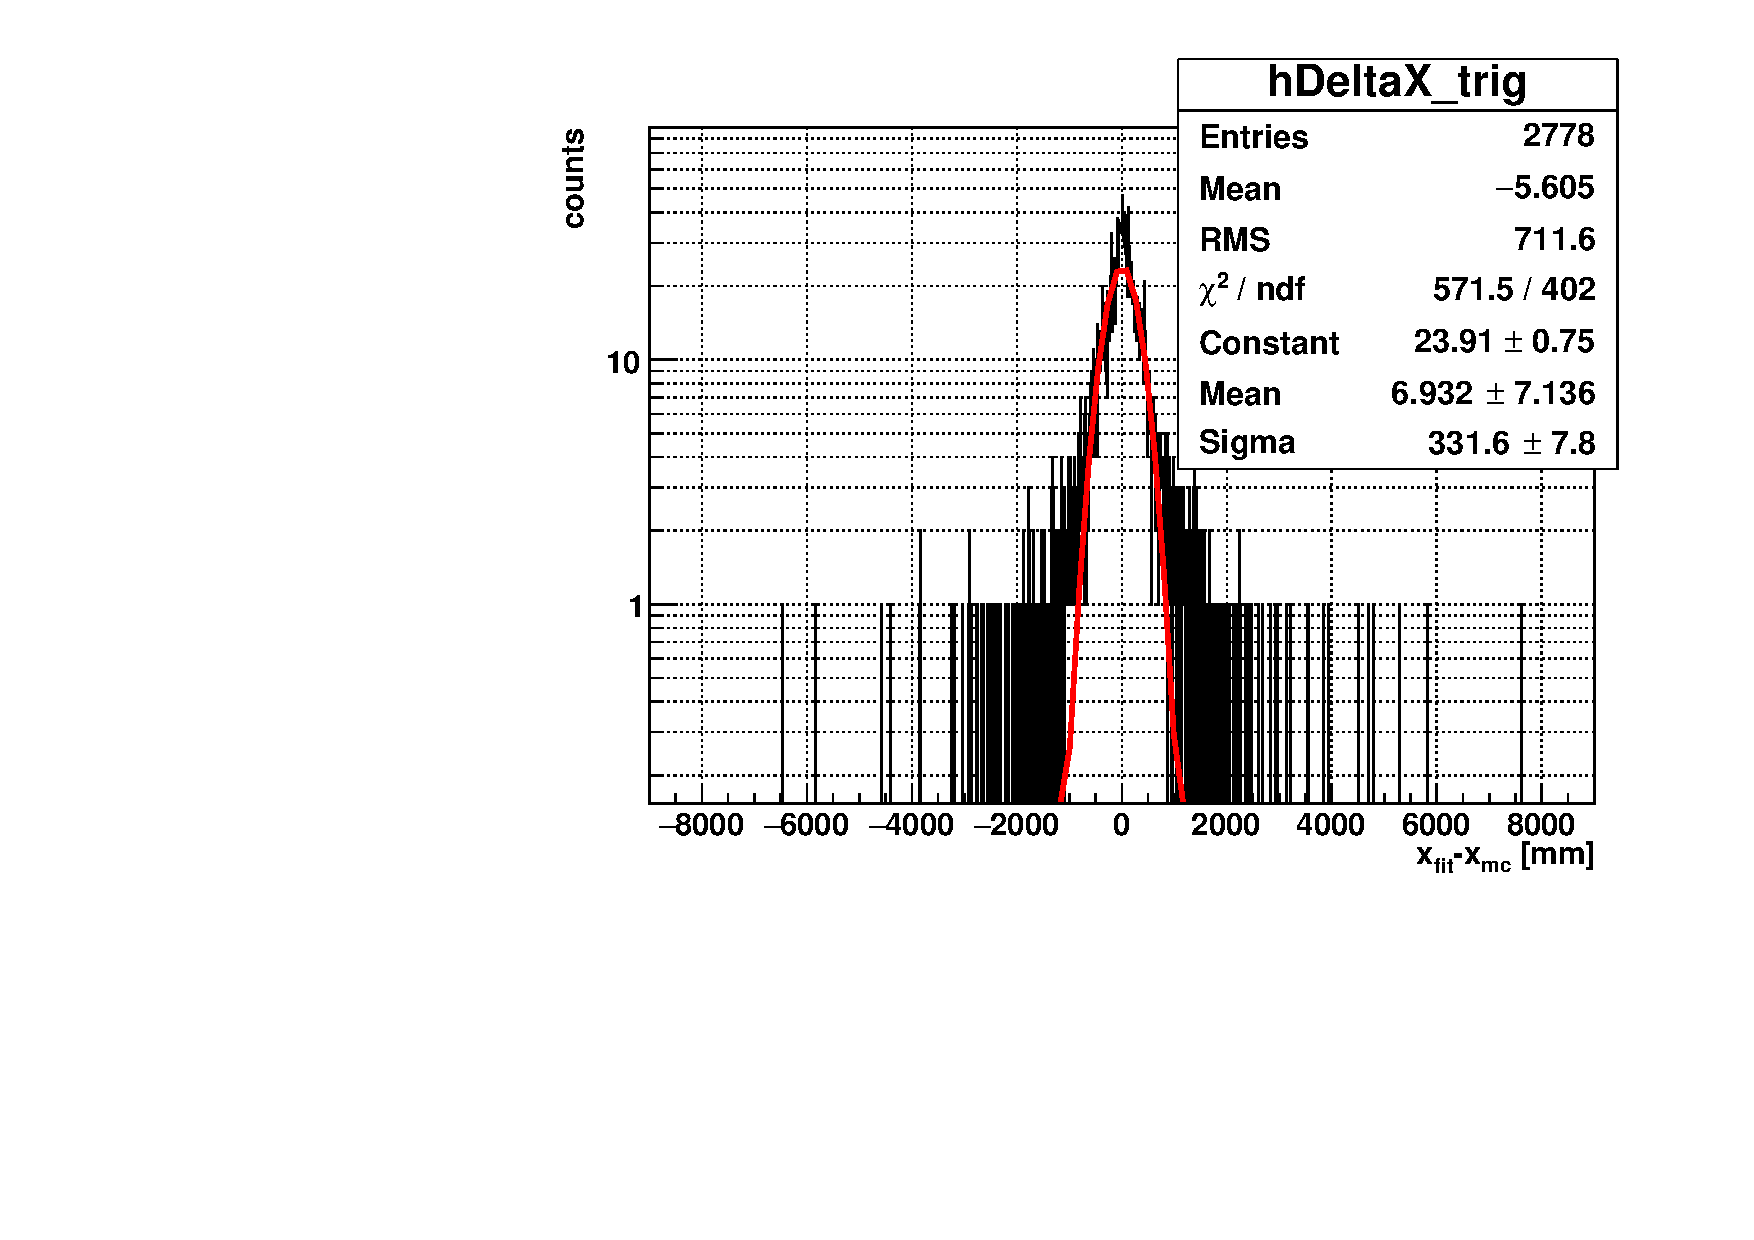
\includegraphics[width=6cm]{partial_full_x.pdf}
		\end{minipage}
	}
	\caption{Distributions of fit position bias projected on x axis ($x_{fit}-x_{MC}$).}
	\label{partial_fit_x}
	\subfigure[scintillator region]{ 
		\begin{minipage}[t]{0.38\textwidth}
			\centering
			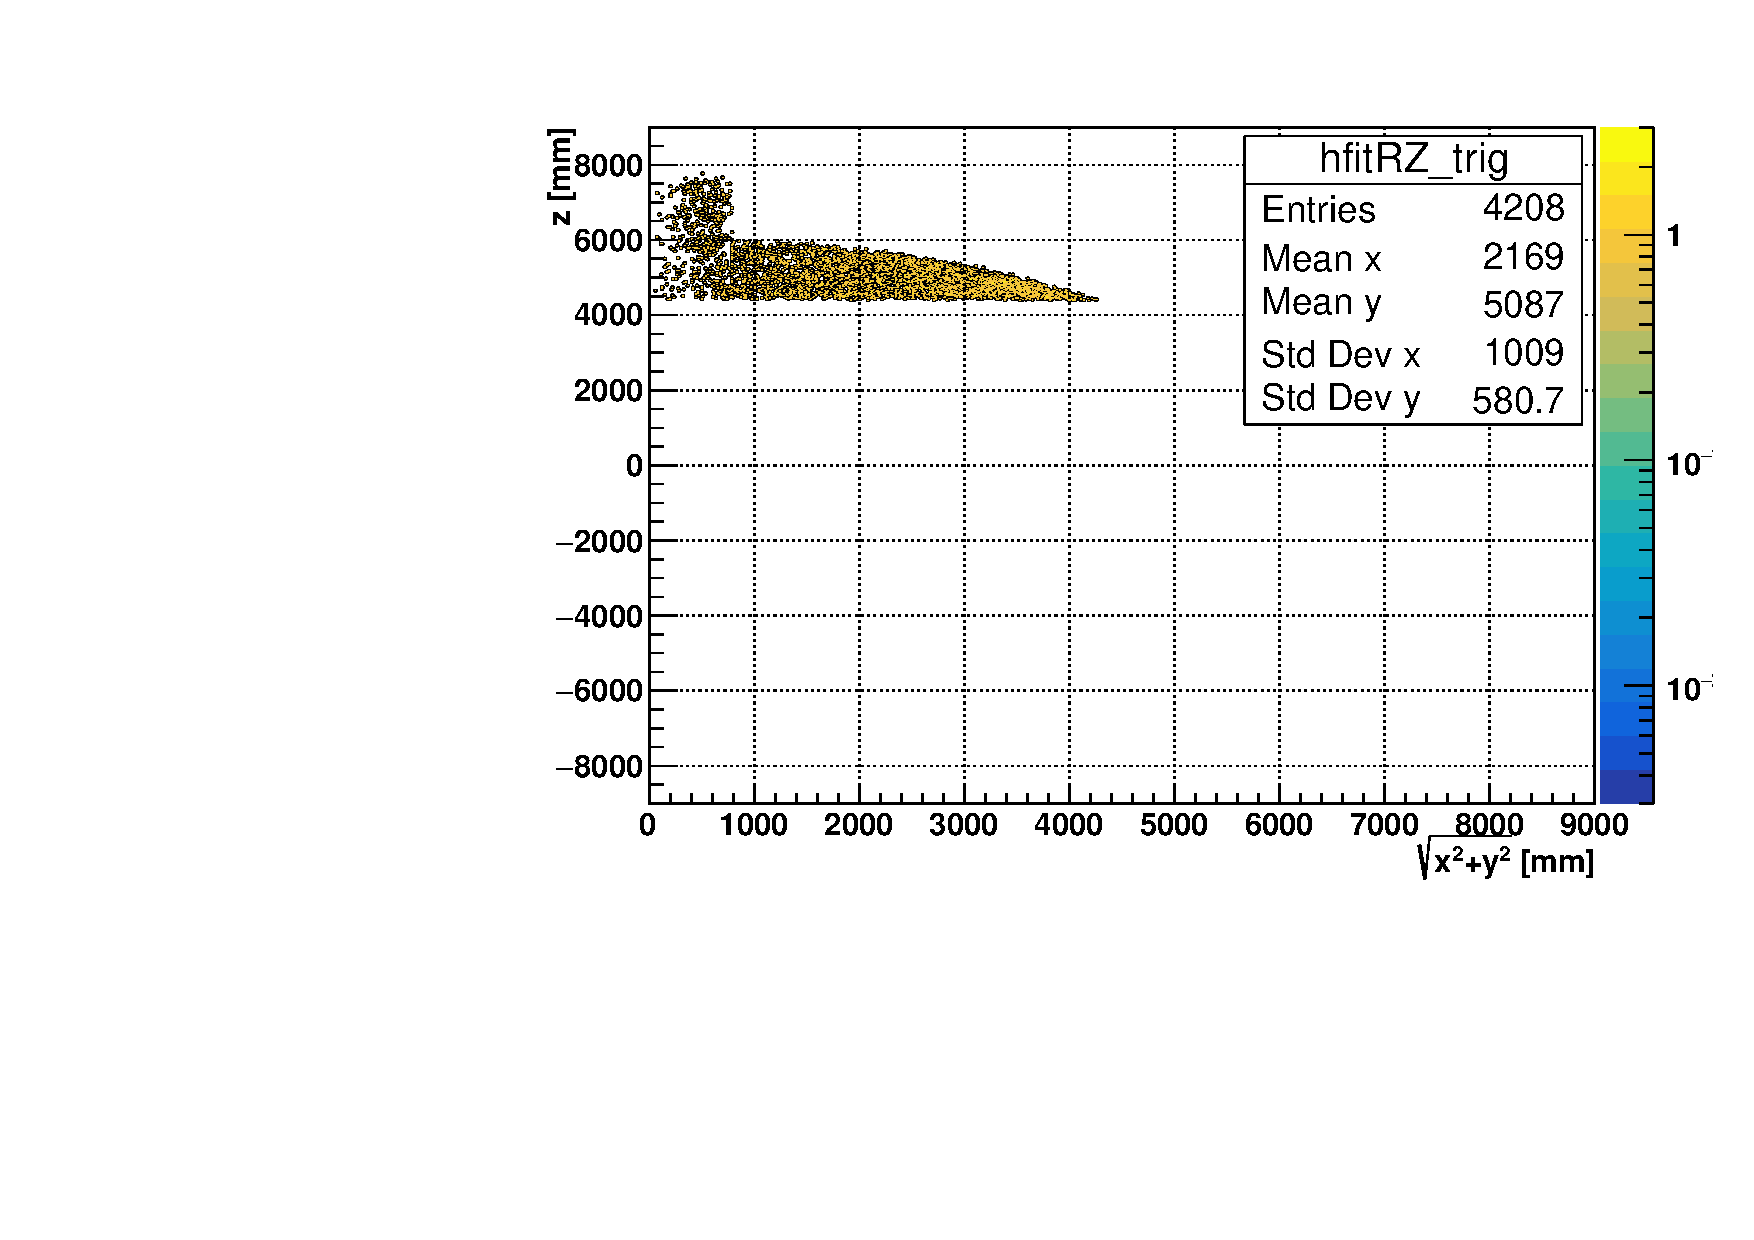
\includegraphics[width=5.8cm]{partial_top_r.pdf}
		\end{minipage}
	}
	\subfigure[water region]{ 
		\begin{minipage}[t]{0.38\textwidth}
			\centering
			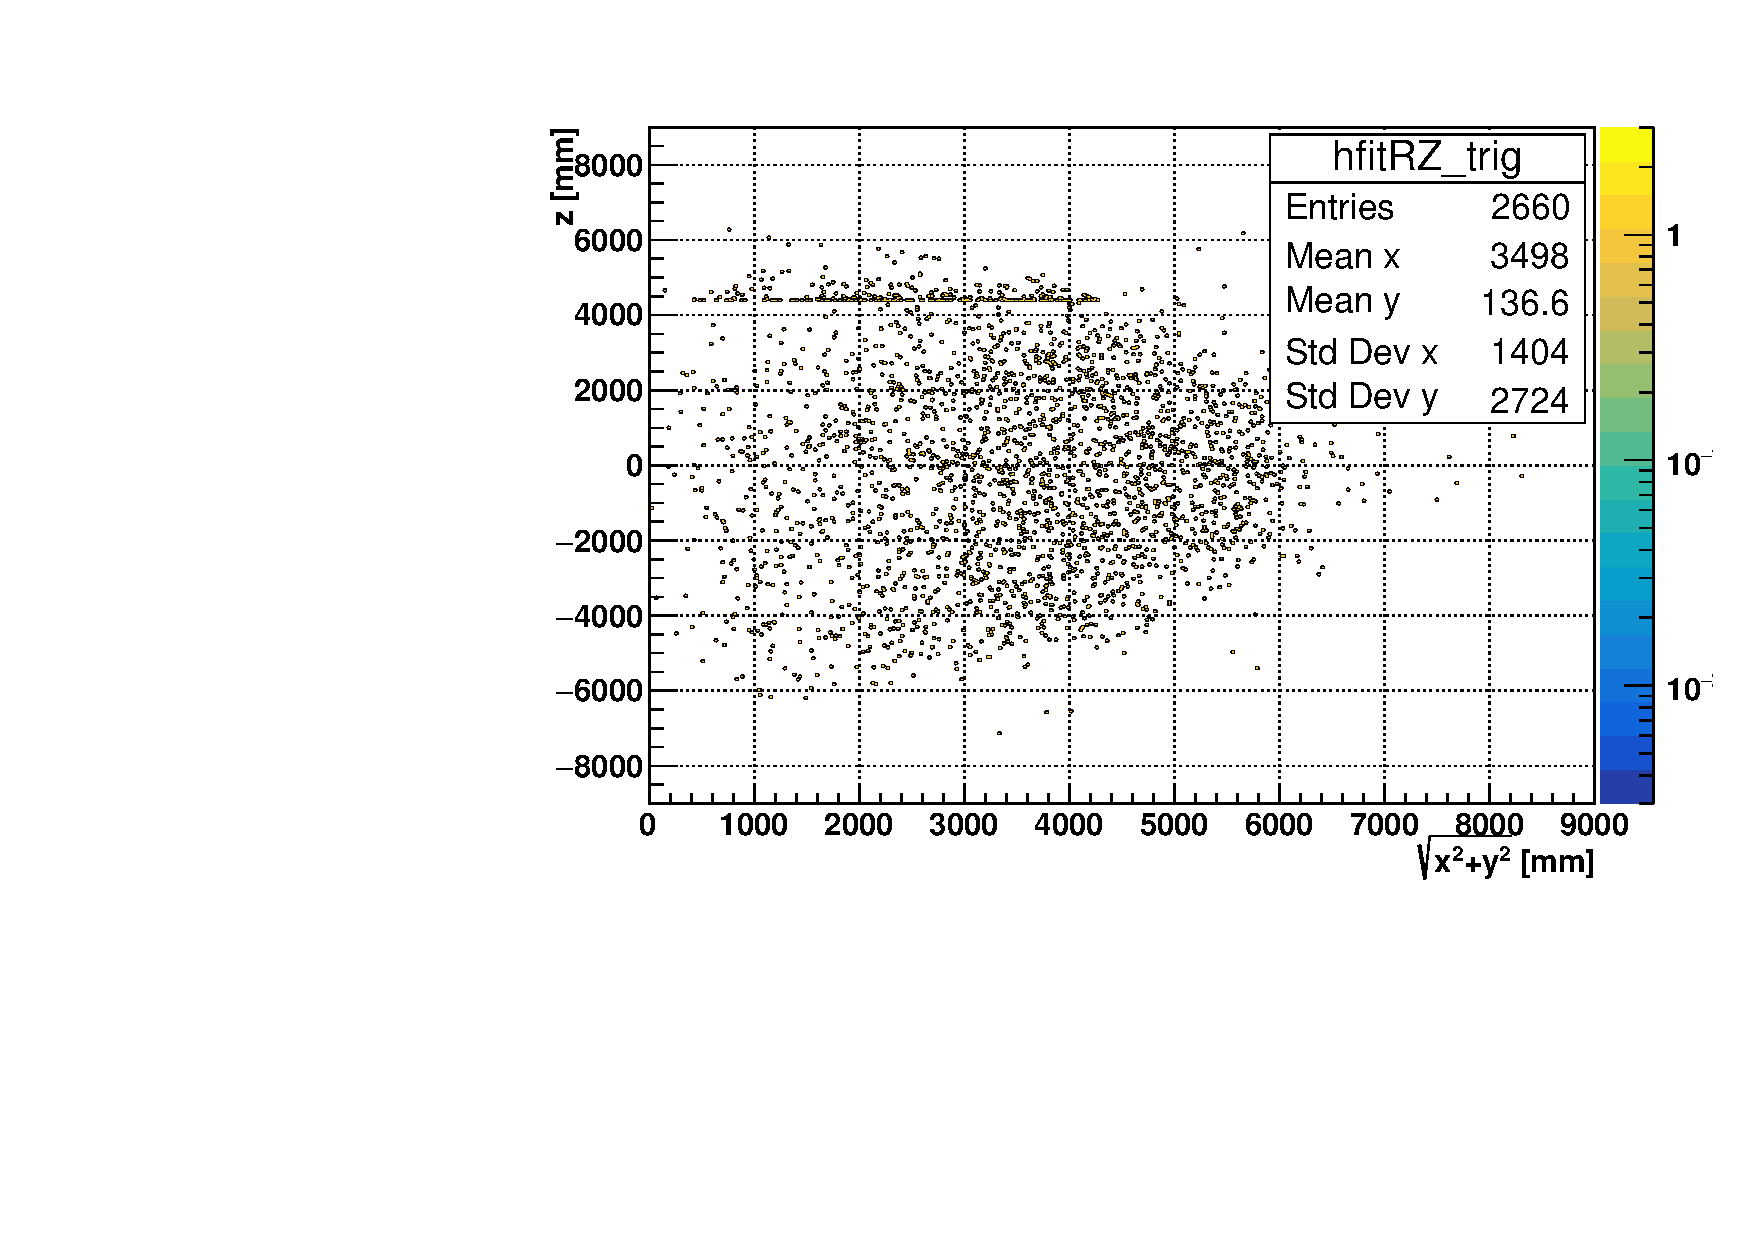
\includegraphics[width=5.8cm]{partial_bot_r.pdf}
		\end{minipage}
	}
	\subfigure[whole region]{ 
		\begin{minipage}[b]{0.35\textwidth}
			\centering
			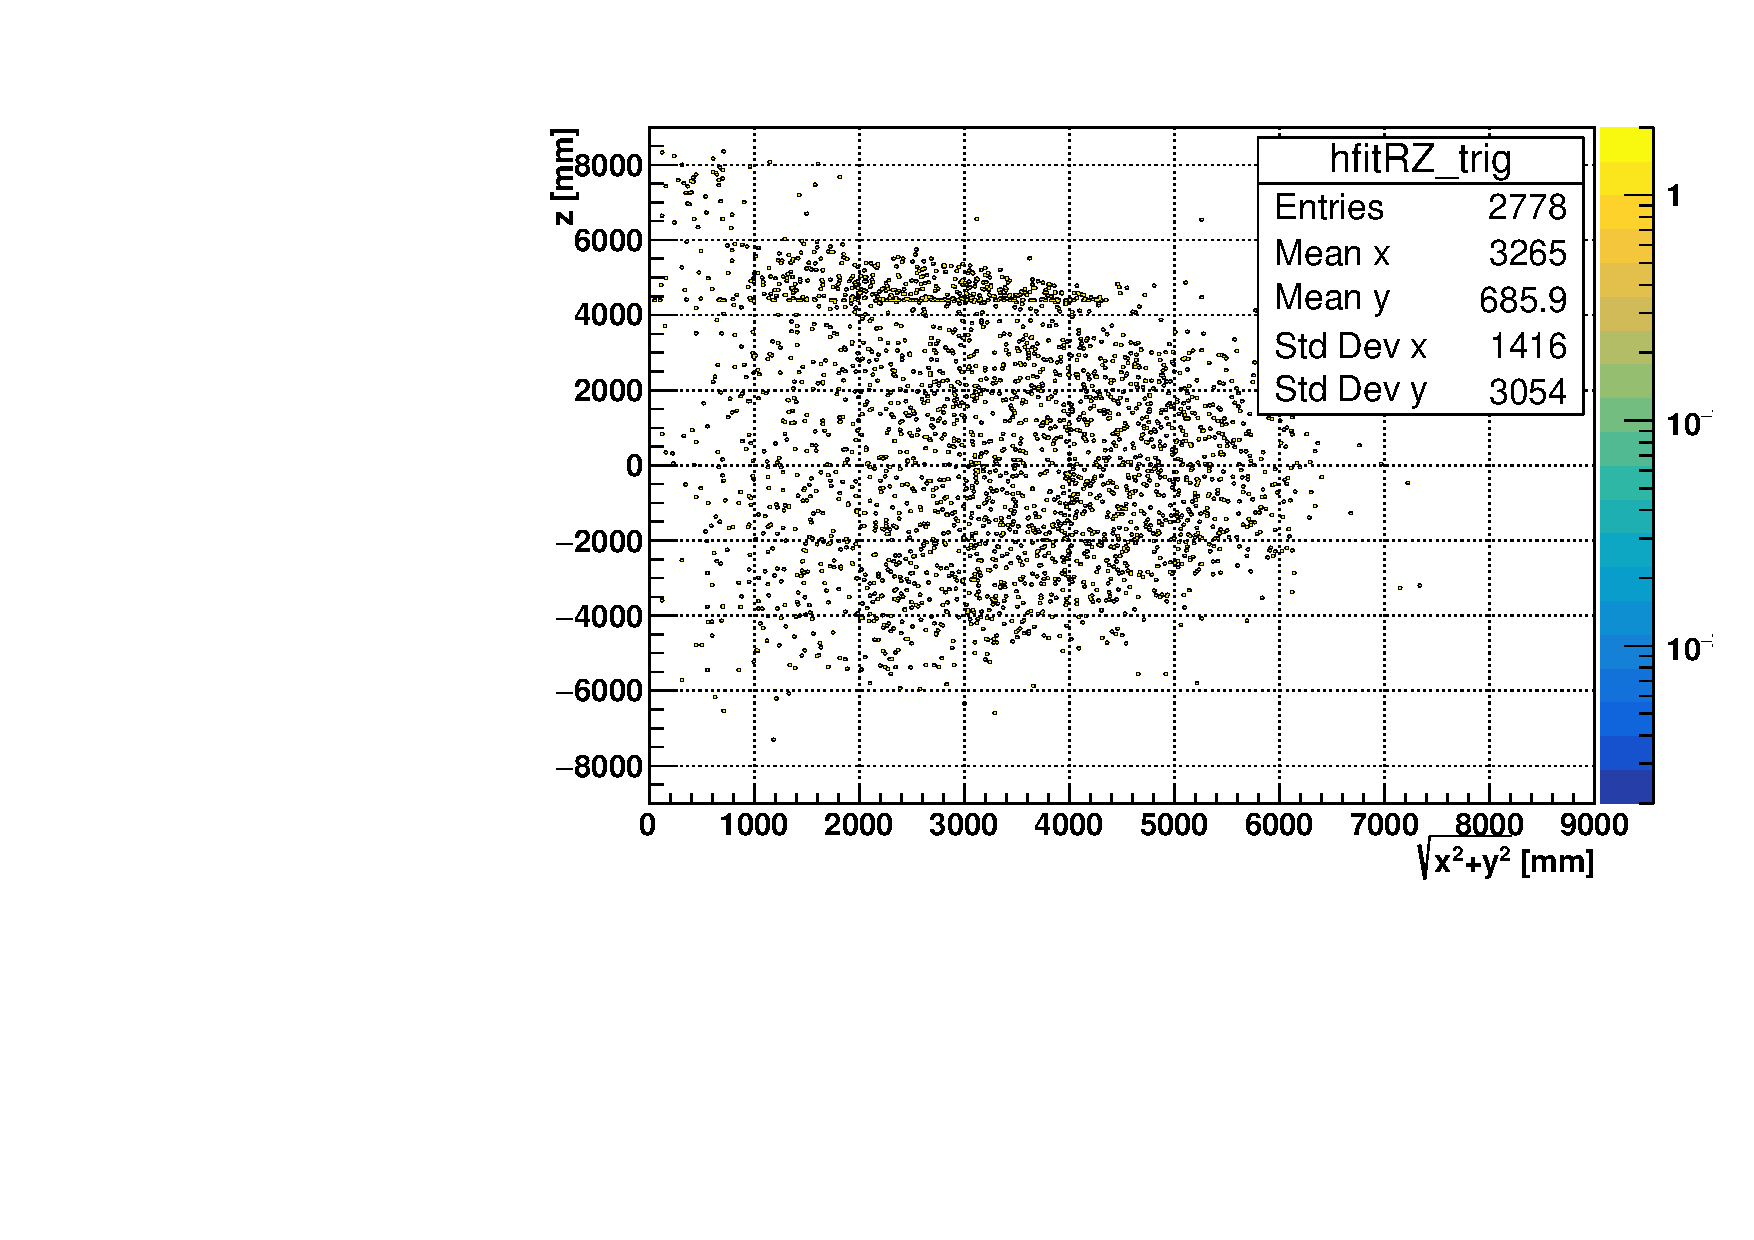
\includegraphics[width=5.8cm]{partial_full_r.pdf}
		\end{minipage}
	}
	\caption{Fit results: $\rho_{fit}=\sqrt{x_{fit}^2+y_{fit}^2}$ vs. $z_{fit}$.}
	\label{partial_fit_rz}
\end{figure}

The performance of the fitter was studied with MC simulations. In a partial fill geometry with water level at 4.435 m, 2.5 MeV electrons are simulated inside the AV in the scintillator region only, the water region only and the whole AV region.

Fig.~\ref{partial_fit_x} and Fig.~\ref{partial_fit_rz} show the MP Partial Fitter reconstructed results for these simulations. Fig.~\ref{partial_fit_x} shows the biases between the fit positions and MC positions, projected on the x axis. The distributions of position biases are fit with Gaussian functions. The values of Gaussian mean and sigma quantify the fit biases and resolutions. Table~\ref{partiaResol} lists these values.

\begin{table}[ht]
	\caption{Reconstructed position biases and resolutions for simulated events in partial fill.}
	\label{partiaResol}
	\centering
	\begin{tabular*}{120mm}{c@{\extracolsep{\fill}}ccc}
		\toprule
		regions of simulated events& bias (mm) &  resolution (mm) \\
		\hline
		scintillator region & -1.0  & 73.9\\
		water region & -10.7 & 385.1\\
		full region &6.9 & 331.72\\
		\bottomrule
	\end{tabular*}
\end{table}
For the events in water, the fit bias and resolution is comparable to the water phase results in Table~\ref{table_posresol}. The events in the scintillator region have smaller fit bias and better resolution due to more hit PMTs in the reconstruction.

Fig.~\ref{partial_fit_rz} shows the fitted $\sqrt{x^2+y^2}$ vs. fitted $z$ positions. It shows that the fitter can distinguish different events in the water or scintillator region. The fitter gives reasonable results of the three different MC simulations. 

pdfs for all timing \ref{sect:LS_SNO+}.


Radial bias is defined as the difference between the fitted and true position, projected along the radial component (unit vector) of the true position \cite{coulter2013modelling}.
\[
(\vec{X}_{fit}-\vec{X}_{true})\cdot \hat{X}_{true}
\]

The value of the mean radial bias is taken by fitting the histogram of the distributions of radial biases with a Gaussian profile and then get the mean of the fitted Gaussian profile.

\subsection{Complicated Situations in Partial-fill}
\subsubsection{Different PPO Concentrations during the Filling}
During the partial-fill phase, the water level and the concentration of PPO were changing.

Oxford group in the SNO+ collaboration has done a few bench-top measurements for the time constants and relative light yields of LAB mixed with different concentrations of PPO\cite{oxfordMeasurement}.

The emission time profiles and relative light yields of PPO dissolved in LAB at the following concentrations: 0.25, 0.5, 1.0, 2.0 and 6.0 g/l.

The partial fitter is re-coordinated according to these measurements.

\begin{table}[ht]
	\centering
	\caption{\label{oxfordMeasure} time constants and amplitudes measured by Oxford group \cite{oxfordMeasurement}.}	
	{\centering
		\begin{tabular*}{160mm}{c@{\extracolsep{\fill}}ccccccccc}
			\toprule 
			PPO [g/L] & $\tau_{rise}$ [ns] & $\tau_1$ [ns] & $\tau_2$ [ns] & $\tau_3$ [ns] & $A_1$ [\%]  & $A_2$ [\%]   & $A_3$ [\%]  & $A'$ [\%] \\
			\midrule
			0.25 & 1.25 & 8.1 & 25.0 & 68.2 & 29.2 & 53.1 & 13.9 & 3.8\\
			0.5  & 1.12 & 7.2 & 18.7 & 49.1 & 43.5 & 40.4 & 12.6 & 3.5 \\
			1.0 & 1.18 & 5.5 & 13.3 & 40.9 &	45.6 & 37.5 & 13.3 & 3.6 \\
			2.0 & 1.06 & 4.2 & 11.7 & 48.9 & 57.9 & 27.8 & 8.9 & 5.4	\\
			6.0 & 0.94 & 2.5 & 9.3  & 46.0 & 63.7 & 17.0 & 8.6 & 10.7\\
			\bottomrule	
		\end{tabular*}
	}
\end{table}


\[
\sum_{i=1}^3 (A_i\frac{e^{-\frac{t}{\tau_i}}-e^{-\frac{t}{\tau_{rise}}}}{\tau_i-\tau_{rise}})+A'\frac{e^{-\frac{t}{\tau_{rise}}}}{\tau_{rise}}
\]

based on these measured parameters, pdfs were built. 

%\begin{figure}[!htb]
%	\centering
%	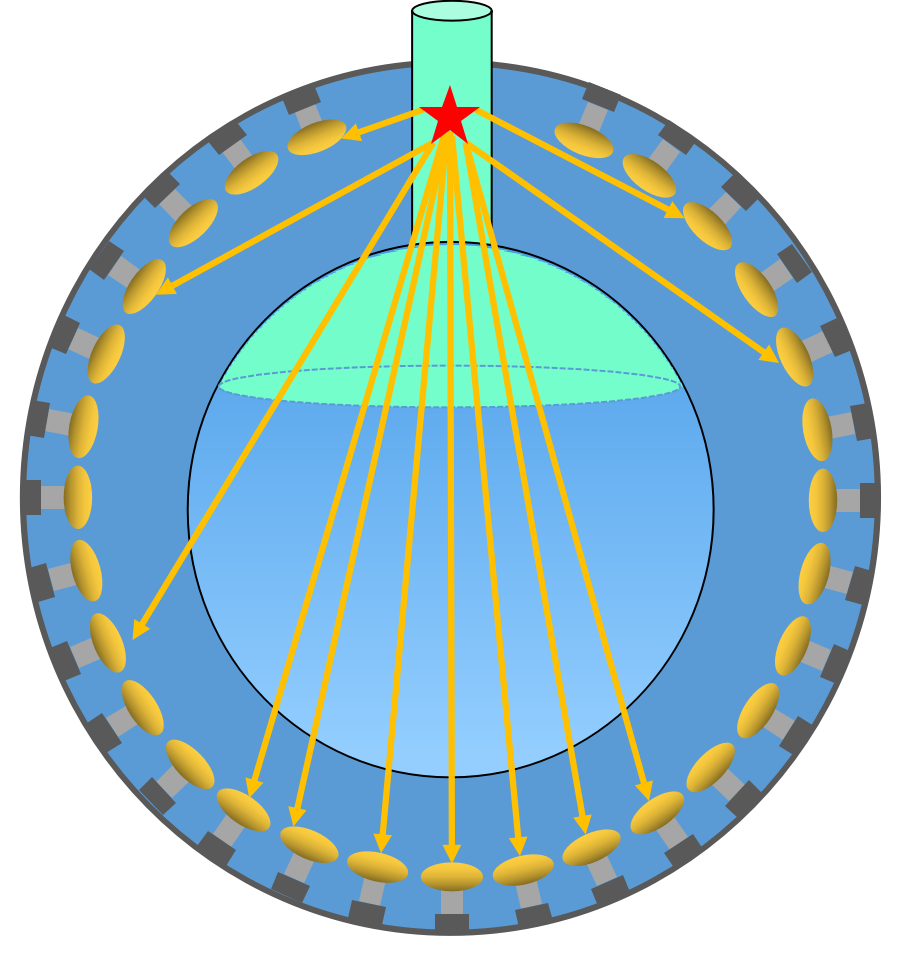
\includegraphics[width=6cm]{skyShine.png}
%	\caption{ Pdfs built for liquid scintillator with various PPO concentrations, based on the bench-top measurements.}
%	\label{oxford_pdf}
%\end{figure}

relative light yield (2g/L = 11900)
\begin{table}[ht]
	\centering
	\caption{\label{oxfordMeasure2}Relative light yield (RLY) measured by \cite{oxfordMeasurement}.}	
	{\centering
		\begin{tabular*}{60mm}{c@{\extracolsep{\fill}}cc}
			\toprule 
			PPO [g/L] & RLY \\
			\midrule
			0.25 & 0.57\\
			0.5 & 0.65\\
			1.0 & 0.9\\
			2.0 & 1.0\\
			6.0 & 0.93\\
			\bottomrule	
		\end{tabular*}
	}
\end{table}

\begin{figure}[!htb]
	\centering
	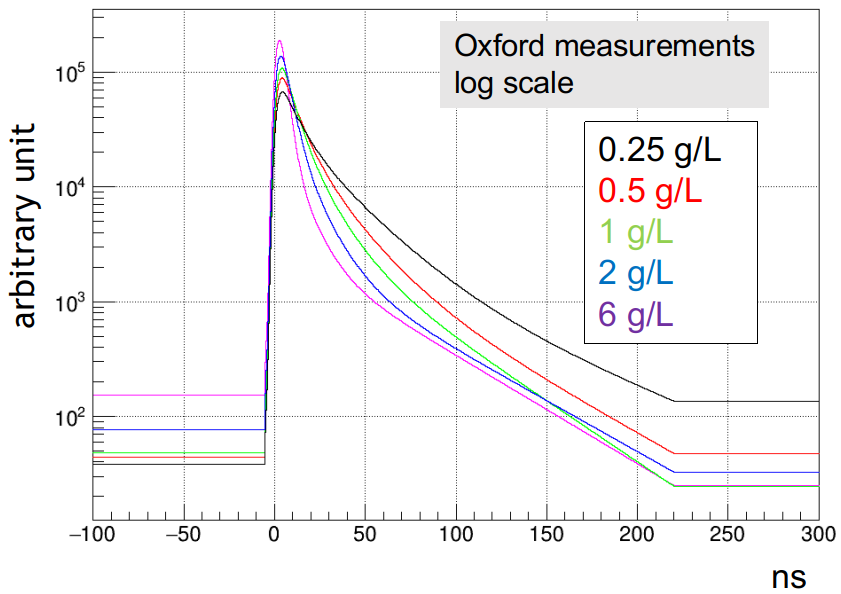
\includegraphics[width=10cm]{oxfordPdf_log.png}
	\caption{Timing spectrum for different PPO concentrations based on the Oxford bench-top measurements.}
	\label{oxfordPdf}
\end{figure}
The partial fitter is invulnerable to the change of pdfs caused by different PPO concentrations.

radial biases
\begin{table}[ht]
	\centering
	\caption{\label{partial_groupV}Tuned effective group velocities for different PPO concentrations.}	
	{\centering
		\begin{tabular*}{140mm}{c@{\extracolsep{\fill}}ccccc}
			\toprule 
			PPO [g/L] & $V_{gr,scint}$ [mm/ns]& $n_{scint}$ & $V_{gr,water}$ [mm/ns]& $n_{water,tuned}$\\
			\midrule
			0.25 & 184.068$\pm$5.153 & 1.629 & 211.871$\pm$5.731 & 1.415\\
			0.5  & 183.467$\pm$5.159 &1.634& 211.587$\pm$-5.773 & 1.417 \\
			1.0 & 182.93$\pm$5.193 &1.639& 211.393$\pm$5.805& 1.418 \\
			2.0 & 183.045$\pm$5.184& 1.638& 211.629$\pm$5.767 & 1.417	\\
			6.0 & 184.218$\pm$5.135& 1.627& 211.173$\pm$5.843 &1.420\\
			\bottomrule	
		\end{tabular*}
	}
\end{table}


Simulate 5000 events for 3 MeV $e^-$,  $\Delta x = x_{fit}-x_{mc}$

\begin{table}[ht]
	\centering
	\caption{\label{partial_bias} Fit speeds and biases for various PPO concentrations.}	
	{\centering
		\begin{tabular*}{145         mm}{c@{\extracolsep{\fill}}cccccc}
			\toprule 
			PPO [g/L] & fit speed [s/event]& $\Delta x$ [mm]& $\Delta y$ [mm]& $\Delta z$ [mm] & $r_{bias}$ [mm] & \\
			\midrule
			0.25 & 0.190 &6.65 &2.64& -18.24& -7.22\\
			0.5  & 0.144 &-0.73 &-1.69& -8.14& 3.30 \\
			1.0 &0.190 & 1.42 &0.57 &-5.65& 10.67 \\
			2.0 &0.194 & 0.34 &1.78& -4.01& 13.37	\\
			6.0 &0.145 & -0.11& -0.12& -25.97& -10.97\\
			\bottomrule	
		\end{tabular*}
	}
\end{table}

%% fit resolutions
$z_{fit}$ resolution [mm] 

%& 120.6
%& 90.02
%& 67.39
%& 55.81
%& 58.62

PPO in Fitter configuration
fit with wrong PPO concentrations:  
\begin{table}[ht]
	\centering
	\caption{\label{partial_bias1} Fit speeds and biases for various PPO concentrations.}	
	{\centering
		\begin{tabular*}{140mm}{c@{\extracolsep{\fill}}cccccccc}
			\toprule 
			PPO [g/L] & $\Delta x$ & $\Delta y$ & $\Delta z$  & $\sigma_z$ & $r_{bias}$  & $\sigma_r$ & ratio in FV (\%)&\\
			\midrule
			0.25 & 6.80& 2.90& -14.61& 121.6& -4.82& 120.3& 93.70\%\\
			0.5  & 5.15& 2.82& -12.85 &120.2 &1.34 &123.0 &93.46\% \\
			1.0 &2.32 &1.95 &-13.22& 120.3& 0.344& 121.9 &93.78\% \\
			2.0 &5.76& 3.03& -9.61& 119.3& 7.264 &125.1& 93.26\% \\
			\bottomrule	
		\end{tabular*}
	}
\end{table}


\subsection{Bi-Po Analysis}
The Bi-Po analysis was performed on simulations to check the fitter efficiency. This analysis suggests a model offset of the water level to include more fitted data.
\begin{figure}[!htb]
	\centering
	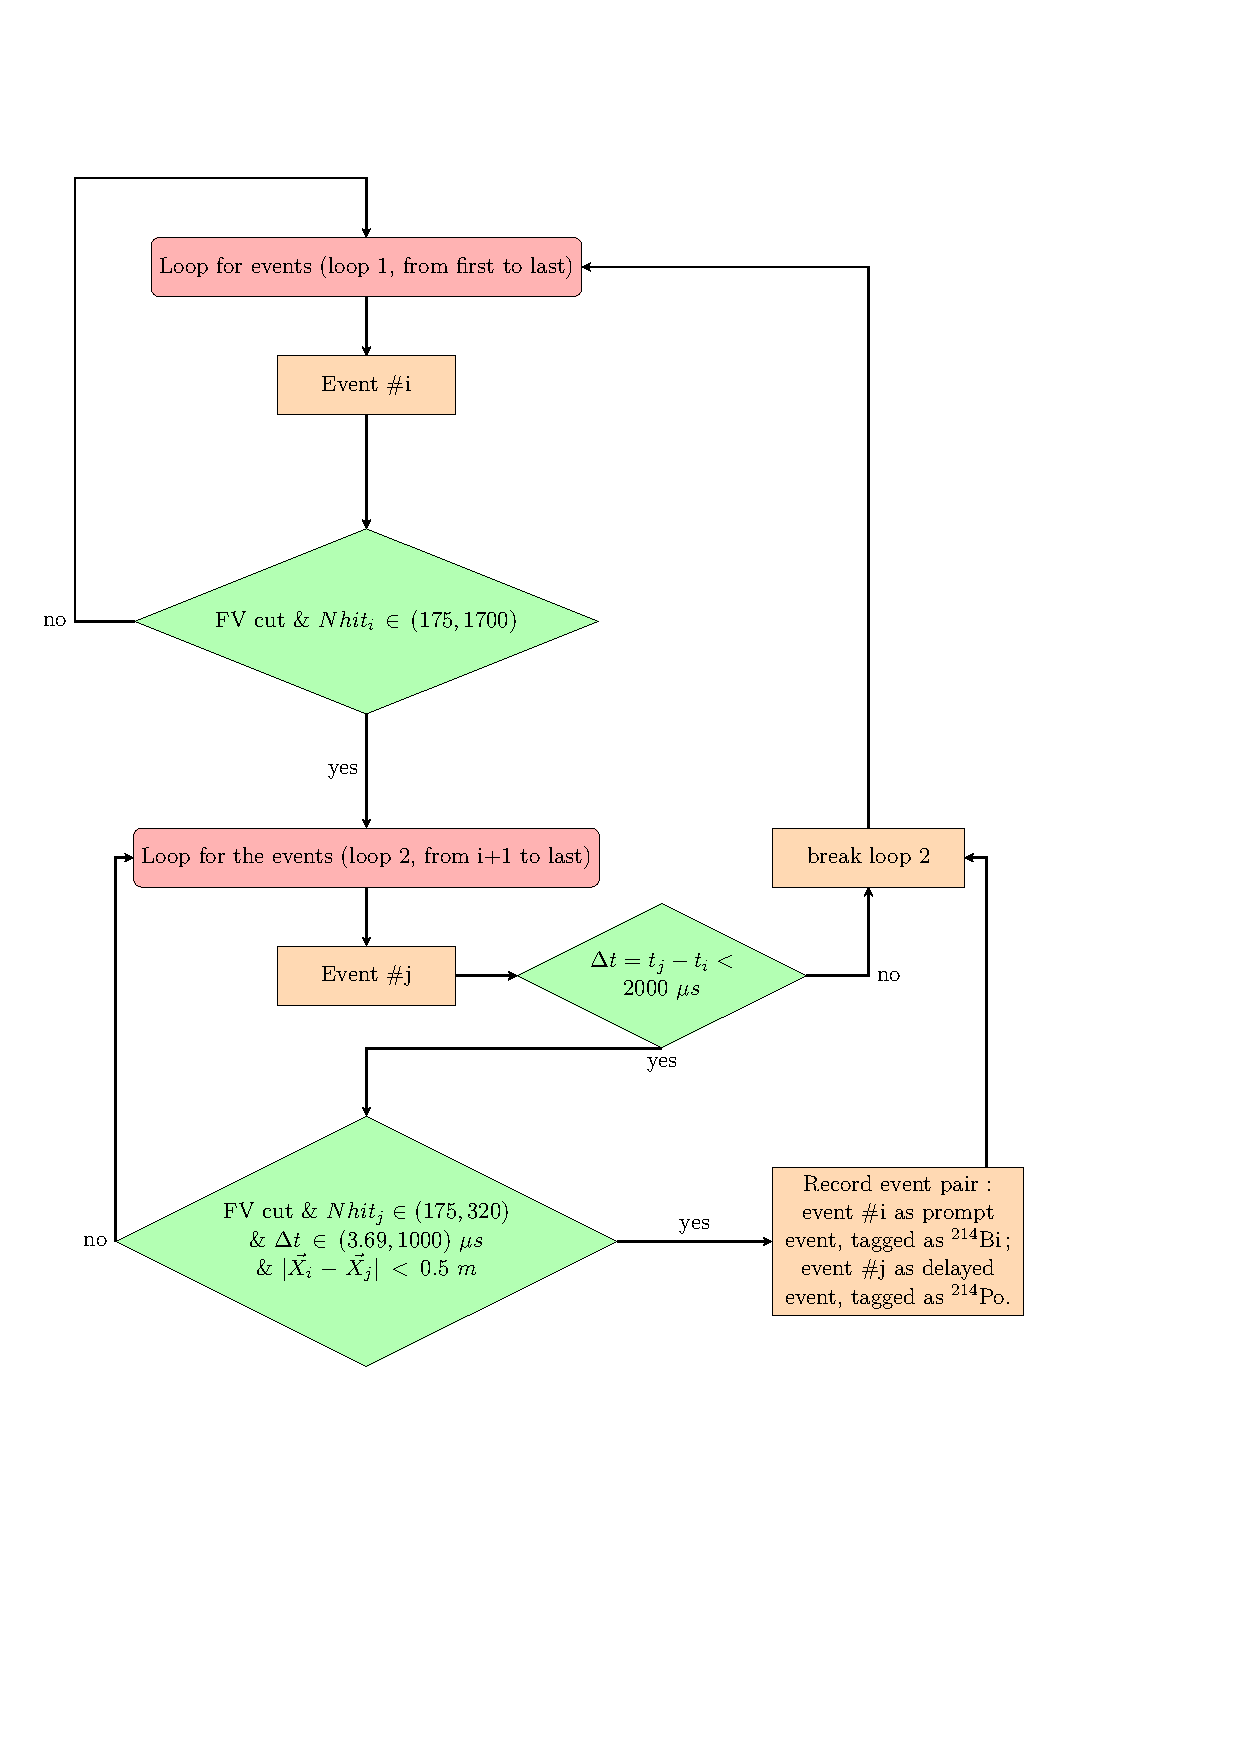
\includegraphics[width=15cm]{flowchart_latex.pdf}
	\caption{A flow chart for Bi-Po tagging.}
	\label{biPo_flowchart}
\end{figure}


\section{PMT Selectors for the Reconstruction}\label{sect:PMTselector}
Several PMT selectors are used to select or remove PMTs from all the recorded PMTs triggered by an event and send the proper PMTs to the fitter for reconstruction. They are developed for optimizing the fitter or boosting up the fit speed:

\begin{itemize}
	\item[$\bullet$] Straight Light Path Time Residual Cut Selector
	
	This selector is used for the direction reconstruction for the SNO+ water phase. It is first developed by Singh for the MultiPath fitter. In the selector, the value of time residual ($t_{res}$) is calculated for each hit PMTs from an event and the PMT with a $t_{res}$ value in a prompt time window of $[-10.0, 120.0]~ns$ is selected for the fitter. The selector calculates $t_{res}$ by using straight line light path, which is the same to the MultiPath water fitter. This can remove the PMTs triggered by photons with late timing, such as the photons reflected off the detector elements (late light) and keep the possible Cherenkov ring hit pattern clear for the direction fitter to fit. Also, dropping the irrelevant PMTs can potentially boost up the fit speed.
	
	\item[$\bullet$] Mode Cut Selector
	
	This selector was developed by the collaboration for all fitters. It checks the hit time ($t_\mathrm{PMT}$) distributions of all the hit PMTs and finds a mode value of the hit time ($t_{mode}$). If $t_{mode}$ fails to be found, it calculates a median value ($t_{median}$) instead\cite{modeCut}. Then it selects the PMT with $t_\mathrm{PMT} \in [t_{mode}+t_{low}, t_{mode}+t_{high}]~ns$. This selector is used to remove the PMTs triggered by noise and light light from reflection. The values of $t_{low},~t_{high}$ are optimized for different scintillators. For the MPW fitter, the optimized window is $[t_{mode}-50, t_{mode}+100]$ ns by checking with the fit biases and resolutions for the \isotope[16]{N} central run data in the water phase, while for the MP scint-water fitter the optimized window is $[t_{mode}-100, t_{mode}+100]$ ns based on checking with the simulations.
	
	\item[$\bullet$] Uniform PMT Selector
	
	I designed this selector for the partial-fill phase and the scintillator phase when a single event can trigger a large amount of PMTs. It reduces the number of the hit PMTs to a designated number ($n_{select}$) in order to boost up the fit speed. When an event triggers $N$ calibrated PMTs, the selector goes through these recorded PMTs and uniformly picks up one PMT by an interval of $\left \lceil{N/n_{select}}\right \rceil $. If $N\leq n_{select}$, the selector does nothing. By doing this, the selector uniformly reduces the number of the PMTs for the fitter without an obvious bias.
	
	\item[$\bullet$] Earliest Hit PMT Selector
	
	Similar to the uniform PMT selector, this selector reduces the number of the hit PMTs to boost up the fit speed. It first groups the PMTs by their positions in the PMT support sphere. Take the centre of the sphere as coordinate origin, the sphere is divided by the azimuth angle $\phi$ (as longitude) and zenith angle $\theta$ (as latitude). In the sphere, the positions of the PMTs in $\phi$, ranging in $[-\pi,\pi]$, is uniformly divided into $n$ intervals while the positions of the PMTs in $\cos\theta$, ranging in $[-1, 1]$, is also divided into $n$ intervals. Thus, the PMTs are grouped into $n\times n$ panels, see Fig.~\ref{GroupPMTs}. 
	\begin{figure}[!htb]
		\centering
		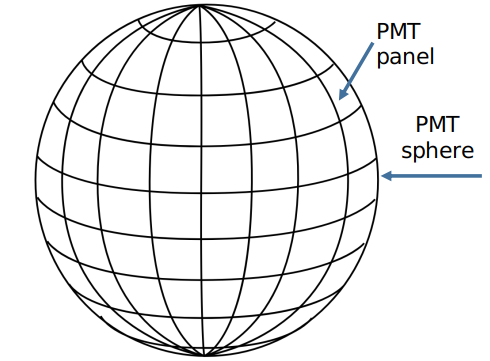
\includegraphics[width=5cm]{GroupPMTs.png}
		\caption{Group the PMTs by dividing the PMT sphere with latitudes and longitudes.}
		\label{GroupPMTs}
	\end{figure}
	
	For each panel, the selector first drops the PMTs triggered too early ($t_\mathrm{PMT}<100~ns$, where $100~ns$ is set as a default threshold). These PMTs could be triggered by noises, such as pre-pulsing. In the rest of the PMTs, the selector picks up one PMT with the earliest $t_\mathrm{PMT}$ in each panel. Thus the number of the PMTs is reduced to $n\times n$ for the fitter, i.e., $n_{select}=n\times n$. If $N\leq n_{select}$, the selector does nothing. 
	
	The other timing parameters can also be used for selecting the PMT in each panel, such as the $t_{mode}$ or the $t_{median}$. However, tests from the simulations for the scintillator phase show that using the earliest hit time gives less fit biases and better fit resolutions.
\end{itemize}

\subsubsection{Water Level}

\[
\frac{\partial L}{\partial splitZ} = \frac{\partial L}{\partial tof}\cdot\frac{\partial tof}{\partial splitZ}=\frac{\partial L}{\partial tof}\cdot\frac{\partial a_3}{\partial splitZ}
\]


\[
\frac{\partial L}{\partial splitZ} = 0
\]


%Appendix: Levenberg-Marquardt method for fitter minimization
(ref: press2007numerical)

%for M unknown parameters: $a_0, a_1, ... , a_{M-1}$ (for example, the 4 parameters of an event vertex: $(x,y,z,t)$)

The pdf can be expanded and fit with Chebyshev polynomials to obtain an analytic approximation function\cite{press2007numerical}. This analytical function can give proper analytical derivatives




\section{Energy Reconstruction}
 
The previous sections mainly focus on vertex and direction reconstruction. For the energy reconstruction in the water phase 

energy response processor, or the energy RSP fitter, is derived from SNO \cite{boulay2004direct,moffat2001optical}.

It uses the fitted position and direction of an event as inputs and then calculates an effective 

estimated $N_\gamma$,

detailed detector effects are taken into account.

the asymmetric geometry of the detector, for example the neck cylinder on the top of the AV sphere; the actual number of online PMTs in a realistic physics run.

\isotope[16]{N} calibration scans at certain detector points.

Energy lookup table built from the simulation data set.

energy look up\cite{energyRSP}.
(energyRSP)

%     A lookup table is used to
%	// map from estimated Cerenkov photons to energy. 
%	
%	the PMT efficiency, and the position and angular dependence of the $NHits$ is also taken into account. 
%	
%	// This method calculates the optical response of each PMT (taking into
%	// account PMT efficiency, solid angle, Cerenkov angular distribution,
%	// etc.) to estimate the number
%	// of Cerenkov photons from the prompt hits. This fitter is only
%	// for a detector geometry with light water in the inner av.


\subsection{Figure of Merit}\label{sect:energy_fom}
Three figure of merit quantities for the energy fitter were developed by the SNO+ collaboration in order to identify the poor reconstructed results which have large biases to the true energy values, especially for the low energy regions around 2.2 MeV, which helps the analysis of neutron capture\cite{waterunidoc}.

%Water Reconstruction Errors & FOMs 6190
\begin{itemize}
	
	\item[$\bullet$]$U$-test ($U_{test}$):
	A Mann-Whitney quantity uses the channel hit probabilities by EneryRSP which are ordered and ranked. The rank of the channels with hits are summed.%cite logan docDB 6190	
		\begin{equation}
		U_{test}\equiv \frac{S-N(N+1)/2}{N(N_{active}-N)},
		\end{equation}
	where $S\equiv \sum_{i}^N \mathrm{rank}_i$. 
	
	\item[$\bullet$] $G$-test ($G_{test}$):
	A quantity uses the hit probabilities by EnergyRSP ($E_i$) which are normalized to the number of observed hits ($N$) %cite logan docDB 6190	
	
	\begin{equation}
	G_{test}\equiv \frac{1}{N}\sum_{i=1}^N \log(\frac{1}{E_i}),
	\end{equation}
	
	\item[$\bullet$] $Z$-factor ($Z_{factor}$):
	A quantity uses the medians and median absolute deviations
of hit probabilities by EnergyRSP
	
	\begin{equation}
     Z'\equiv 1-\frac{3(\sigma_p+\sigma_n)}{\mu_p-\mu_n},
    \end{equation}
\end{itemize}

\subsection{Energy Reconstruction in Partial-fill Phase}
Up till this thesis writing, there is no proper energy fitter for the partial-fill phase works. I attempted two methods for the energy reconstruction in the partial-fill phase: the NHit scale method and the NHit ratio method. Both of them are based on the simulations. These two methods need more effects to be improved.
\subsubsection{NHit Scale}
In the partial-fill phase ,  In \cite{partialEnergy}, 
to scale $NHits$ based on several sets of simulations.

\subsubsection{NHit Ratio}

The fitter follows the idea of the charge-ratio fitter for the partial energy reconstruction\cite{partialEnergyYang}.

\begin{equation}
E = p_0+p_1\cdot NHit+p_2\cdot NHit^2
\end{equation}


NHit ratio table based on position.


\section{Other Reconstruction Algorithms}
\subsection{Hough Transformation for Direction Reconstruction}

Hough transformation is a pattern recognition algorithm used in image analysis and computer vision\cite{davies1997machine}. This algorithm was first invent to extract patterns in bubble chamber\cite{houghwiki}, 

is used by Super-K\cite{shiozawa1999reconstruction}.

The Hough transformation algorithm was used in SNO data analysis for counting the numbers of the Cherenkov rings caused by multiple charged particles in a high energy event such as atmospheric neutrinos event\cite{bonventre2014neutron}. It is also suggested for the reconstruction of event direction in the SNO+ scintillator phase\cite{houghTransform}.

As illustrated in Fig.~\ref{houghTrans}, 


circular Hough transformation
\begin{figure}[!htb]
	\centering
	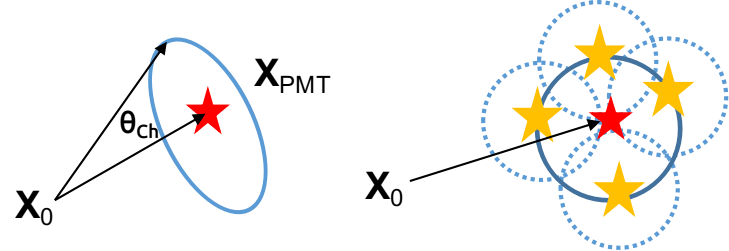
\includegraphics[width=8cm]{houghTransform.png}
	\caption{Hough transformation for catching the ring structure of Cherenkov signals and fitting the direction.}
	\label{houghTrans}
\end{figure}

\subsection{Reconstructions Based on the Deep Learning}
The vast amount of data collected by the particle detectors make it feasible to implement machine learning algorithms for data analysis.
The machine learning algorithms, such as 

artificial neural network (ANN), have been implemented into the data analysis as well as the event reconstruction in SNO+. In the RAT software, an ANN position reconstruction algorithm (position ANN) has been developed and will be implemented in future. 

This algorithm trains the neural network from calibration data to find the position of an event.

At the time of this writing, a few machine learning or deep learning algorithms are being developed. Based on the PMT hit patterns.

Learning from the simulations as well as the calibration data, 

and then predicts the event position and direction.

utilize the computing power of the graphics processing unit (GPU). 
Once a neural network is trained, 
inference is very fast.

Traditional approach can fail to converge
parallelize

the deep learning framework is being developed.
and to aid data analysis
100x - 1,000x quicker on CPU (Central Processing Unit)
10,000 times quicker on GPU .
\cite{markNeuralNetwork,markNeuralTalk}.

\section{Conclusion}
The Multi-path Fitter framework of event vertex reconstruction was developed for multiple SNO+ physics phases. Under this framework, the \texttt{Multi-path Water Fitter} works as an alternative fitter to provide additional reconstruction information for the water data and it gives proper position and direction resolutions for the water analysis. The \texttt{Multi-path Scint-Water Fitter} works as the prime fitter for the SNO+ partial-fill phase.